\documentclass[11pt]{article}
\usepackage{amsmath,amssymb}
\usepackage{graphicx}
\usepackage{longtable}
\usepackage{array}
\usepackage{xurl}
\usepackage[hidelinks]{hyperref}
\usepackage[margin=0.9in]{geometry}
\usepackage[numbers]{natbib}
% Generated by reapschema.report; do not edit.
% config: paper
% results-hash: 417e9e5c49a26c543e409a6946ec791e31a37543321074b43a488199275cfc8d
\newcommand{\AccCurrentCleanEeiMare}{31.2}
\newcommand{\AccCurrentCleanEeiMedian}{22.8}
\newcommand{\AccCurrentCleanEeiQHigh}{100.1}
\newcommand{\AccCurrentCleanEeiQLow}{2.0}
\newcommand{\AccCurrentCleanEeiShareTen}{74.9}
\newcommand{\AccCurrentCleanResMare}{0.4}
\newcommand{\AccCurrentCleanResMedian}{0.33}
\newcommand{\AccCurrentCleanResQHigh}{0.98}
\newcommand{\AccCurrentCleanResQLow}{0.03}
\newcommand{\AccCurrentCleanResShareTen}{0.0}
\newcommand{\AccCurrentUnvalidatedEeiMare}{36.5}
\newcommand{\AccCurrentUnvalidatedEeiMedian}{25.5}
\newcommand{\AccCurrentUnvalidatedEeiQHigh}{228.4}
\newcommand{\AccCurrentUnvalidatedEeiQLow}{2.1}
\newcommand{\AccCurrentUnvalidatedEeiShareTen}{76.6}
\newcommand{\AccCurrentUnvalidatedResMare}{8.3}
\newcommand{\AccCurrentUnvalidatedResMedian}{0.40}
\newcommand{\AccCurrentUnvalidatedResQHigh}{69.43}
\newcommand{\AccCurrentUnvalidatedResQLow}{0.04}
\newcommand{\AccCurrentUnvalidatedResShareTen}{13.7}
\newcommand{\AccCurrentValidatedEeiMare}{33.4}
\newcommand{\AccCurrentValidatedEeiMedian}{23.8}
\newcommand{\AccCurrentValidatedEeiQHigh}{130.3}
\newcommand{\AccCurrentValidatedEeiQLow}{2.0}
\newcommand{\AccCurrentValidatedEeiShareTen}{75.5}
\newcommand{\AccCurrentValidatedResMare}{1.0}
\newcommand{\AccCurrentValidatedResMedian}{0.35}
\newcommand{\AccCurrentValidatedResQHigh}{1.24}
\newcommand{\AccCurrentValidatedResQLow}{0.03}
\newcommand{\AccCurrentValidatedResShareTen}{2.6}
\newcommand{\AccDatesCleanEeiMare}{30.7}
\newcommand{\AccDatesCleanEeiMedian}{22.5}
\newcommand{\AccDatesCleanEeiQHigh}{97.3}
\newcommand{\AccDatesCleanEeiQLow}{2.0}
\newcommand{\AccDatesCleanEeiShareTen}{75.0}
\newcommand{\AccDatesCleanResMare}{0.4}
\newcommand{\AccDatesCleanResMedian}{0.33}
\newcommand{\AccDatesCleanResQHigh}{0.98}
\newcommand{\AccDatesCleanResQLow}{0.03}
\newcommand{\AccDatesCleanResShareTen}{0.0}
\newcommand{\AccDatesNormCleanEeiMare}{23.1}
\newcommand{\AccDatesNormCleanEeiMedian}{15.2}
\newcommand{\AccDatesNormCleanEeiQHigh}{76.8}
\newcommand{\AccDatesNormCleanEeiQLow}{1.1}
\newcommand{\AccDatesNormCleanEeiShareTen}{63.9}
\newcommand{\AccDatesNormCleanResMare}{0.4}
\newcommand{\AccDatesNormCleanResMedian}{0.33}
\newcommand{\AccDatesNormCleanResQHigh}{0.98}
\newcommand{\AccDatesNormCleanResQLow}{0.03}
\newcommand{\AccDatesNormCleanResShareTen}{0.0}
\newcommand{\AccDatesNormReadCleanEeiMare}{21.5}
\newcommand{\AccDatesNormReadCleanEeiMedian}{14.5}
\newcommand{\AccDatesNormReadCleanEeiQHigh}{69.3}
\newcommand{\AccDatesNormReadCleanEeiQLow}{1.1}
\newcommand{\AccDatesNormReadCleanEeiShareTen}{61.9}
\newcommand{\AccDatesNormReadCleanResMare}{0.4}
\newcommand{\AccDatesNormReadCleanResMedian}{0.33}
\newcommand{\AccDatesNormReadCleanResQHigh}{0.98}
\newcommand{\AccDatesNormReadCleanResQLow}{0.03}
\newcommand{\AccDatesNormReadCleanResShareTen}{0.0}
\newcommand{\AccDatesNormReadUnvalidatedEeiMare}{27.9}
\newcommand{\AccDatesNormReadUnvalidatedEeiMedian}{16.3}
\newcommand{\AccDatesNormReadUnvalidatedEeiQHigh}{226.9}
\newcommand{\AccDatesNormReadUnvalidatedEeiQLow}{1.1}
\newcommand{\AccDatesNormReadUnvalidatedEeiShareTen}{64.7}
\newcommand{\AccDatesNormReadUnvalidatedResMare}{8.3}
\newcommand{\AccDatesNormReadUnvalidatedResMedian}{0.40}
\newcommand{\AccDatesNormReadUnvalidatedResQHigh}{69.43}
\newcommand{\AccDatesNormReadUnvalidatedResQLow}{0.04}
\newcommand{\AccDatesNormReadUnvalidatedResShareTen}{13.7}
\newcommand{\AccDatesNormReadValidatedEeiMare}{24.3}
\newcommand{\AccDatesNormReadValidatedEeiMedian}{15.2}
\newcommand{\AccDatesNormReadValidatedEeiQHigh}{102.0}
\newcommand{\AccDatesNormReadValidatedEeiQLow}{1.1}
\newcommand{\AccDatesNormReadValidatedEeiShareTen}{63.1}
\newcommand{\AccDatesNormReadValidatedResMare}{1.0}
\newcommand{\AccDatesNormReadValidatedResMedian}{0.35}
\newcommand{\AccDatesNormReadValidatedResQHigh}{1.24}
\newcommand{\AccDatesNormReadValidatedResQLow}{0.03}
\newcommand{\AccDatesNormReadValidatedResShareTen}{2.6}
\newcommand{\AccDatesNormUnvalidatedEeiMare}{29.5}
\newcommand{\AccDatesNormUnvalidatedEeiMedian}{17.2}
\newcommand{\AccDatesNormUnvalidatedEeiQHigh}{245.6}
\newcommand{\AccDatesNormUnvalidatedEeiQLow}{1.3}
\newcommand{\AccDatesNormUnvalidatedEeiShareTen}{66.7}
\newcommand{\AccDatesNormUnvalidatedResMare}{8.3}
\newcommand{\AccDatesNormUnvalidatedResMedian}{0.40}
\newcommand{\AccDatesNormUnvalidatedResQHigh}{69.43}
\newcommand{\AccDatesNormUnvalidatedResQLow}{0.04}
\newcommand{\AccDatesNormUnvalidatedResShareTen}{13.7}
\newcommand{\AccDatesNormValidatedEeiMare}{25.9}
\newcommand{\AccDatesNormValidatedEeiMedian}{16.2}
\newcommand{\AccDatesNormValidatedEeiQHigh}{117.2}
\newcommand{\AccDatesNormValidatedEeiQLow}{1.2}
\newcommand{\AccDatesNormValidatedEeiShareTen}{65.0}
\newcommand{\AccDatesNormValidatedResMare}{1.0}
\newcommand{\AccDatesNormValidatedResMedian}{0.35}
\newcommand{\AccDatesNormValidatedResQHigh}{1.24}
\newcommand{\AccDatesNormValidatedResQLow}{0.03}
\newcommand{\AccDatesNormValidatedResShareTen}{2.6}
\newcommand{\AccDatesUnvalidatedEeiMare}{36.1}
\newcommand{\AccDatesUnvalidatedEeiMedian}{25.0}
\newcommand{\AccDatesUnvalidatedEeiQHigh}{227.0}
\newcommand{\AccDatesUnvalidatedEeiQLow}{2.1}
\newcommand{\AccDatesUnvalidatedEeiShareTen}{76.6}
\newcommand{\AccDatesUnvalidatedResMare}{8.3}
\newcommand{\AccDatesUnvalidatedResMedian}{0.40}
\newcommand{\AccDatesUnvalidatedResQHigh}{69.43}
\newcommand{\AccDatesUnvalidatedResQLow}{0.04}
\newcommand{\AccDatesUnvalidatedResShareTen}{13.7}
\newcommand{\AccDatesValidatedEeiMare}{33.1}
\newcommand{\AccDatesValidatedEeiMedian}{23.5}
\newcommand{\AccDatesValidatedEeiQHigh}{130.3}
\newcommand{\AccDatesValidatedEeiQLow}{2.0}
\newcommand{\AccDatesValidatedEeiShareTen}{75.7}
\newcommand{\AccDatesValidatedResMare}{1.0}
\newcommand{\AccDatesValidatedResMedian}{0.35}
\newcommand{\AccDatesValidatedResQHigh}{1.24}
\newcommand{\AccDatesValidatedResQLow}{0.03}
\newcommand{\AccDatesValidatedResShareTen}{2.6}
\newcommand{\AccIntervalCleanEeiMare}{18.6}
\newcommand{\AccIntervalCleanEeiMedian}{12.1}
\newcommand{\AccIntervalCleanEeiQHigh}{60.3}
\newcommand{\AccIntervalCleanEeiQLow}{0.9}
\newcommand{\AccIntervalCleanEeiShareTen}{55.6}
\newcommand{\AccIntervalCleanResMare}{0.4}
\newcommand{\AccIntervalCleanResMedian}{0.33}
\newcommand{\AccIntervalCleanResQHigh}{0.98}
\newcommand{\AccIntervalCleanResQLow}{0.03}
\newcommand{\AccIntervalCleanResShareTen}{0.0}
\newcommand{\AccIntervalUnvalidatedEeiMare}{18.6}
\newcommand{\AccIntervalUnvalidatedEeiMedian}{12.1}
\newcommand{\AccIntervalUnvalidatedEeiQHigh}{60.3}
\newcommand{\AccIntervalUnvalidatedEeiQLow}{0.9}
\newcommand{\AccIntervalUnvalidatedEeiShareTen}{55.6}
\newcommand{\AccIntervalUnvalidatedResMare}{0.4}
\newcommand{\AccIntervalUnvalidatedResMedian}{0.33}
\newcommand{\AccIntervalUnvalidatedResQHigh}{0.98}
\newcommand{\AccIntervalUnvalidatedResQLow}{0.03}
\newcommand{\AccIntervalUnvalidatedResShareTen}{0.0}
\newcommand{\AccIntervalValidatedEeiMare}{18.6}
\newcommand{\AccIntervalValidatedEeiMedian}{12.1}
\newcommand{\AccIntervalValidatedEeiQHigh}{60.3}
\newcommand{\AccIntervalValidatedEeiQLow}{0.9}
\newcommand{\AccIntervalValidatedEeiShareTen}{55.6}
\newcommand{\AccIntervalValidatedResMare}{0.4}
\newcommand{\AccIntervalValidatedResMedian}{0.33}
\newcommand{\AccIntervalValidatedResQHigh}{0.98}
\newcommand{\AccIntervalValidatedResQLow}{0.03}
\newcommand{\AccIntervalValidatedResShareTen}{0.0}
\newcommand{\AccMetadataCleanEeiMare}{21.5}
\newcommand{\AccMetadataCleanEeiMedian}{14.5}
\newcommand{\AccMetadataCleanEeiQHigh}{69.3}
\newcommand{\AccMetadataCleanEeiQLow}{1.1}
\newcommand{\AccMetadataCleanEeiShareTen}{61.9}
\newcommand{\AccMetadataCleanResMare}{0.4}
\newcommand{\AccMetadataCleanResMedian}{0.33}
\newcommand{\AccMetadataCleanResQHigh}{0.98}
\newcommand{\AccMetadataCleanResQLow}{0.03}
\newcommand{\AccMetadataCleanResShareTen}{0.0}
\newcommand{\AccMetadataUnvalidatedEeiMare}{27.9}
\newcommand{\AccMetadataUnvalidatedEeiMedian}{16.3}
\newcommand{\AccMetadataUnvalidatedEeiQHigh}{226.9}
\newcommand{\AccMetadataUnvalidatedEeiQLow}{1.1}
\newcommand{\AccMetadataUnvalidatedEeiShareTen}{64.7}
\newcommand{\AccMetadataUnvalidatedResMare}{4.2}
\newcommand{\AccMetadataUnvalidatedResMedian}{0.35}
\newcommand{\AccMetadataUnvalidatedResQHigh}{1.36}
\newcommand{\AccMetadataUnvalidatedResQLow}{0.03}
\newcommand{\AccMetadataUnvalidatedResShareTen}{3.9}
\newcommand{\AccMetadataValidatedEeiMare}{21.5}
\newcommand{\AccMetadataValidatedEeiMedian}{14.5}
\newcommand{\AccMetadataValidatedEeiQHigh}{69.3}
\newcommand{\AccMetadataValidatedEeiQLow}{1.1}
\newcommand{\AccMetadataValidatedEeiShareTen}{61.8}
\newcommand{\AccMetadataValidatedResMare}{0.4}
\newcommand{\AccMetadataValidatedResMedian}{0.34}
\newcommand{\AccMetadataValidatedResQHigh}{0.99}
\newcommand{\AccMetadataValidatedResQLow}{0.03}
\newcommand{\AccMetadataValidatedResShareTen}{0.0}
\newcommand{\AccNettingCleanEeiMare}{31.2}
\newcommand{\AccNettingCleanEeiMedian}{22.8}
\newcommand{\AccNettingCleanEeiQHigh}{100.1}
\newcommand{\AccNettingCleanEeiQLow}{2.0}
\newcommand{\AccNettingCleanEeiShareTen}{74.9}
\newcommand{\AccNettingCleanResMare}{0.4}
\newcommand{\AccNettingCleanResMedian}{0.33}
\newcommand{\AccNettingCleanResQHigh}{0.98}
\newcommand{\AccNettingCleanResQLow}{0.03}
\newcommand{\AccNettingCleanResShareTen}{0.0}
\newcommand{\AccNettingUnvalidatedEeiMare}{36.5}
\newcommand{\AccNettingUnvalidatedEeiMedian}{25.5}
\newcommand{\AccNettingUnvalidatedEeiQHigh}{228.4}
\newcommand{\AccNettingUnvalidatedEeiQLow}{2.1}
\newcommand{\AccNettingUnvalidatedEeiShareTen}{76.6}
\newcommand{\AccNettingUnvalidatedResMare}{8.3}
\newcommand{\AccNettingUnvalidatedResMedian}{0.40}
\newcommand{\AccNettingUnvalidatedResQHigh}{69.43}
\newcommand{\AccNettingUnvalidatedResQLow}{0.04}
\newcommand{\AccNettingUnvalidatedResShareTen}{13.7}
\newcommand{\AccNettingValidatedEeiMare}{33.4}
\newcommand{\AccNettingValidatedEeiMedian}{23.8}
\newcommand{\AccNettingValidatedEeiQHigh}{130.3}
\newcommand{\AccNettingValidatedEeiQLow}{2.0}
\newcommand{\AccNettingValidatedEeiShareTen}{75.5}
\newcommand{\AccNettingValidatedResMare}{1.0}
\newcommand{\AccNettingValidatedResMedian}{0.35}
\newcommand{\AccNettingValidatedResQHigh}{1.23}
\newcommand{\AccNettingValidatedResQLow}{0.03}
\newcommand{\AccNettingValidatedResShareTen}{2.5}
\newcommand{\AccProductionMeterCleanEeiMare}{31.2}
\newcommand{\AccProductionMeterCleanEeiMedian}{22.8}
\newcommand{\AccProductionMeterCleanEeiQHigh}{100.1}
\newcommand{\AccProductionMeterCleanEeiQLow}{2.0}
\newcommand{\AccProductionMeterCleanEeiShareTen}{74.9}
\newcommand{\AccProductionMeterCleanResMare}{0.4}
\newcommand{\AccProductionMeterCleanResMedian}{0.33}
\newcommand{\AccProductionMeterCleanResQHigh}{0.98}
\newcommand{\AccProductionMeterCleanResQLow}{0.03}
\newcommand{\AccProductionMeterCleanResShareTen}{0.0}
\newcommand{\AccProductionMeterUnvalidatedEeiMare}{36.5}
\newcommand{\AccProductionMeterUnvalidatedEeiMedian}{25.5}
\newcommand{\AccProductionMeterUnvalidatedEeiQHigh}{228.4}
\newcommand{\AccProductionMeterUnvalidatedEeiQLow}{2.1}
\newcommand{\AccProductionMeterUnvalidatedEeiShareTen}{76.6}
\newcommand{\AccProductionMeterUnvalidatedResMare}{4.2}
\newcommand{\AccProductionMeterUnvalidatedResMedian}{0.35}
\newcommand{\AccProductionMeterUnvalidatedResQHigh}{1.36}
\newcommand{\AccProductionMeterUnvalidatedResQLow}{0.03}
\newcommand{\AccProductionMeterUnvalidatedResShareTen}{3.9}
\newcommand{\AccProductionMeterValidatedEeiMare}{33.4}
\newcommand{\AccProductionMeterValidatedEeiMedian}{23.8}
\newcommand{\AccProductionMeterValidatedEeiQHigh}{130.3}
\newcommand{\AccProductionMeterValidatedEeiQLow}{2.0}
\newcommand{\AccProductionMeterValidatedEeiShareTen}{75.5}
\newcommand{\AccProductionMeterValidatedResMare}{0.4}
\newcommand{\AccProductionMeterValidatedResMedian}{0.34}
\newcommand{\AccProductionMeterValidatedResQHigh}{0.99}
\newcommand{\AccProductionMeterValidatedResQLow}{0.03}
\newcommand{\AccProductionMeterValidatedResShareTen}{0.0}
\newcommand{\AnchorMinutes}{161}
\newcommand{\AnchorResponses}{2}
\newcommand{\AucBillDiffGrossNet}{0.80}
\newcommand{\AucBillDiffUnlabGrossNet}{0.65}
\newcommand{\AucOutlierTransposed}{0.54}
\newcommand{\AucPlausGeomNameplate}{0.97}
\newcommand{\AucPlausGrossNet}{0.96}
\newcommand{\AucPlausNameplate}{0.96}
\newcommand{\AucShapeTransposed}{0.57}
\newcommand{\AuditChainedHours}{150{,}153}
\newcommand{\AuditChainedShortfall}{730}
\newcommand{\AuditHoursDiscrepancy}{705}
\newcommand{\AuditHoursDiscrepancyPct}{0.47}
\newcommand{\AuditHoursPerRespondent}{50.7}
\newcommand{\AuditHoursPerResponse}{1.34}
\newcommand{\AuditImpliedHoursPerResponse}{1.3463}
\newcommand{\AuditImpliedResponsesPerRespondent}{37.6463}
\newcommand{\AuditProductHours}{150{,}178}
\newcommand{\AuditProductResponses}{112{,}054}
\newcommand{\AuditRespondents}{2{,}977}
\newcommand{\AuditResponses}{112{,}073}
\newcommand{\AuditResponsesDiscrepancy}{19}
\newcommand{\AuditResponsesPerRespondent}{37.64}
\newcommand{\AuditRoundedHoursPerResponse}{1.35}
\newcommand{\AuditRoundedResponsesPerRespondent}{37.65}
\newcommand{\AuditTotalHours}{150{,}883}
\newcommand{\AwardFitADCritical}{0.75}
\newcommand{\AwardFitADEei}{5.0}
\newcommand{\AwardFitADRes}{35.0}
\newcommand{\AwardFitNEei}{573}
\newcommand{\AwardFitNRes}{1{,}745}
\newcommand{\AwardShareAtSmallCap}{17}
\newcommand{\BandHighEdge}{20}
\newcommand{\BandHighIntervalPathMedian}{13}
\newcommand{\BandHighN}{860}
\newcommand{\BandHighNormMedian}{15}
\newcommand{\BandHighUndatedMedian}{17}
\newcommand{\BandLowEdge}{10}
\newcommand{\BandLowIntervalPathMedian}{15}
\newcommand{\BandLowN}{1{,}760}
\newcommand{\BandLowNormMedian}{19}
\newcommand{\BandLowUndatedMedian}{33}
\newcommand{\BandMidIntervalPathMedian}{9}
\newcommand{\BandMidN}{1{,}837}
\newcommand{\BandMidNormMedian}{13}
\newcommand{\BandMidUndatedMedian}{19}
\newcommand{\BaseBurden}{166}
\newcommand{\BaseFlagRate}{12}
\newcommand{\BaseMare}{8.2}
\newcommand{\BaseMareSe}{0.14}
\newcommand{\BaseSel}{9.2}
\newcommand{\BasisComstockIntervalMedian}{8}
\newcommand{\BasisComstockN}{2{,}239}
\newcommand{\BasisComstockNormMedian}{10}
\newcommand{\BasisComstockUndatedMedian}{19}
\newcommand{\BasisHypotheticalIntervalMedian}{18}
\newcommand{\BasisHypotheticalN}{2{,}218}
\newcommand{\BasisHypotheticalNormMedian}{20}
\newcommand{\BasisHypotheticalUndatedMedian}{27}
\newcommand{\CfgAreCap}{1}
\newcommand{\CfgBootstrap}{1{,}000}
\newcommand{\CfgBootstrapBlock}{3}
\newcommand{\CfgConfidence}{90}
\newcommand{\CfgCvrmseMax}{25}
\newcommand{\CfgDailyNoise}{6}
\newcommand{\CfgEstimatedProb}{5}
\newcommand{\CfgFundingRatio}{35}
\newcommand{\CfgGridHigh}{90}
\newcommand{\CfgGridLow}{30}
\newcommand{\CfgGridStep}{3}
\newcommand{\CfgMcDraws}{2{,}000}
\newcommand{\CfgMeterError}{0.5}
\newcommand{\CfgMinNonzero}{3}
\newcommand{\CfgOccupancyProb}{15}
\newcommand{\CfgPvTolAnnual}{3}
\newcommand{\CfgPvTolMonthly}{6}
\newcommand{\CfgRateDouble}{4}
\newcommand{\CfgRateGrossNet}{5}
\newcommand{\CfgRateNameplate}{5}
\newcommand{\CfgRatePeriod}{5}
\newcommand{\CfgRateTransposed}{5}
\newcommand{\CfgRateUnit}{4}
\newcommand{\CfgReserveShare}{20}
\newcommand{\CfgSeed}{20261130}
\newcommand{\CfgTopPerState}{2}
\newcommand{\ChangeHoursPct}{41}
\newcommand{\ChangeHoursPerResponsePct}{57}
\newcommand{\ChangeRespondentsPct}{35}
\newcommand{\ChangeResponsesPct}{37}
\newcommand{\ChangeResponsesPerRespondentFactor}{2.1}
\newcommand{\ConvRelSeCurrent}{1.7}
\newcommand{\ConvRelSeRec}{1.9}
\newcommand{\CoverageBootstrap}{74}
\newcommand{\CoverageFsu}{88}
\newcommand{\CoverageN}{457}
\newcommand{\CoverageNominal}{90}
\newcommand{\DatesNormBurden}{184}
\newcommand{\DatesNormBurdenIncrease}{18}
\newcommand{\DatesNormBurdenIncreasePct}{11}
\newcommand{\DatesNormMare}{6.6}
\newcommand{\DatesNormMareReductionPct}{20}
\newcommand{\DetCurrentEeiDouble}{2}
\newcommand{\DetCurrentEeiFalsePositive}{5.1}
\newcommand{\DetCurrentEeiPeriod}{6}
\newcommand{\DetCurrentEeiPpv}{58}
\newcommand{\DetCurrentEeiRecall}{32}
\newcommand{\DetCurrentEeiTransposed}{29}
\newcommand{\DetCurrentEeiUnit}{100}
\newcommand{\DetCurrentResDouble}{2}
\newcommand{\DetCurrentResFalsePositive}{1.6}
\newcommand{\DetCurrentResGrossNet}{88}
\newcommand{\DetCurrentResNameplate}{42}
\newcommand{\DetCurrentResPeriod}{2}
\newcommand{\DetCurrentResPpv}{91}
\newcommand{\DetCurrentResRecall}{42}
\newcommand{\DetCurrentResTransposed}{22}
\newcommand{\DetCurrentResUnit}{100}
\newcommand{\DetDatesEeiDouble}{3}
\newcommand{\DetDatesEeiFalsePositive}{5.6}
\newcommand{\DetDatesEeiPeriod}{100}
\newcommand{\DetDatesEeiPpv}{70}
\newcommand{\DetDatesEeiRecall}{59}
\newcommand{\DetDatesEeiTransposed}{30}
\newcommand{\DetDatesEeiUnit}{100}
\newcommand{\DetDatesNormEeiDouble}{3}
\newcommand{\DetDatesNormEeiFalsePositive}{5.6}
\newcommand{\DetDatesNormEeiPeriod}{100}
\newcommand{\DetDatesNormEeiPpv}{70}
\newcommand{\DetDatesNormEeiRecall}{59}
\newcommand{\DetDatesNormEeiTransposed}{30}
\newcommand{\DetDatesNormEeiUnit}{100}
\newcommand{\DetDatesNormReadEeiDouble}{3}
\newcommand{\DetDatesNormReadEeiFalsePositive}{5.6}
\newcommand{\DetDatesNormReadEeiPeriod}{100}
\newcommand{\DetDatesNormReadEeiPpv}{70}
\newcommand{\DetDatesNormReadEeiRecall}{59}
\newcommand{\DetDatesNormReadEeiTransposed}{30}
\newcommand{\DetDatesNormReadEeiUnit}{100}
\newcommand{\DetDatesNormReadResDouble}{2}
\newcommand{\DetDatesNormReadResFalsePositive}{1.9}
\newcommand{\DetDatesNormReadResGrossNet}{88}
\newcommand{\DetDatesNormReadResNameplate}{42}
\newcommand{\DetDatesNormReadResPeriod}{100}
\newcommand{\DetDatesNormReadResPpv}{93}
\newcommand{\DetDatesNormReadResRecall}{60}
\newcommand{\DetDatesNormReadResTransposed}{22}
\newcommand{\DetDatesNormReadResUnit}{100}
\newcommand{\DetDatesNormResDouble}{2}
\newcommand{\DetDatesNormResFalsePositive}{1.9}
\newcommand{\DetDatesNormResGrossNet}{88}
\newcommand{\DetDatesNormResNameplate}{42}
\newcommand{\DetDatesNormResPeriod}{100}
\newcommand{\DetDatesNormResPpv}{93}
\newcommand{\DetDatesNormResRecall}{60}
\newcommand{\DetDatesNormResTransposed}{22}
\newcommand{\DetDatesNormResUnit}{100}
\newcommand{\DetDatesResDouble}{2}
\newcommand{\DetDatesResFalsePositive}{1.9}
\newcommand{\DetDatesResGrossNet}{88}
\newcommand{\DetDatesResNameplate}{42}
\newcommand{\DetDatesResPeriod}{100}
\newcommand{\DetDatesResPpv}{93}
\newcommand{\DetDatesResRecall}{60}
\newcommand{\DetDatesResTransposed}{22}
\newcommand{\DetDatesResUnit}{100}
\newcommand{\DetIntervalEeiDouble}{2}
\newcommand{\DetIntervalEeiFalsePositive}{5.1}
\newcommand{\DetIntervalEeiPeriod}{6}
\newcommand{\DetIntervalEeiPpv}{58}
\newcommand{\DetIntervalEeiRecall}{32}
\newcommand{\DetIntervalEeiTransposed}{29}
\newcommand{\DetIntervalEeiUnit}{100}
\newcommand{\DetIntervalResDouble}{2}
\newcommand{\DetIntervalResFalsePositive}{1.6}
\newcommand{\DetIntervalResGrossNet}{88}
\newcommand{\DetIntervalResNameplate}{42}
\newcommand{\DetIntervalResPeriod}{2}
\newcommand{\DetIntervalResPpv}{91}
\newcommand{\DetIntervalResRecall}{42}
\newcommand{\DetIntervalResTransposed}{22}
\newcommand{\DetIntervalResUnit}{100}
\newcommand{\DetMetadataEeiDouble}{100}
\newcommand{\DetMetadataEeiFalsePositive}{5.6}
\newcommand{\DetMetadataEeiPeriod}{100}
\newcommand{\DetMetadataEeiPpv}{76}
\newcommand{\DetMetadataEeiRecall}{80}
\newcommand{\DetMetadataEeiTransposed}{30}
\newcommand{\DetMetadataEeiUnit}{100}
\newcommand{\DetMetadataResDouble}{100}
\newcommand{\DetMetadataResFalsePositive}{4.8}
\newcommand{\DetMetadataResGrossNet}{99}
\newcommand{\DetMetadataResNameplate}{98}
\newcommand{\DetMetadataResPeriod}{100}
\newcommand{\DetMetadataResPpv}{88}
\newcommand{\DetMetadataResRecall}{90}
\newcommand{\DetMetadataResTransposed}{45}
\newcommand{\DetMetadataResUnit}{100}
\newcommand{\DetNettingEeiDouble}{2}
\newcommand{\DetNettingEeiFalsePositive}{5.1}
\newcommand{\DetNettingEeiPeriod}{6}
\newcommand{\DetNettingEeiPpv}{58}
\newcommand{\DetNettingEeiRecall}{32}
\newcommand{\DetNettingEeiTransposed}{29}
\newcommand{\DetNettingEeiUnit}{100}
\newcommand{\DetNettingResDouble}{2}
\newcommand{\DetNettingResFalsePositive}{3.2}
\newcommand{\DetNettingResGrossNet}{89}
\newcommand{\DetNettingResNameplate}{43}
\newcommand{\DetNettingResPeriod}{4}
\newcommand{\DetNettingResPpv}{84}
\newcommand{\DetNettingResRecall}{43}
\newcommand{\DetNettingResTransposed}{24}
\newcommand{\DetNettingResUnit}{100}
\newcommand{\DetProductionMeterEeiDouble}{2}
\newcommand{\DetProductionMeterEeiFalsePositive}{5.1}
\newcommand{\DetProductionMeterEeiPeriod}{6}
\newcommand{\DetProductionMeterEeiPpv}{58}
\newcommand{\DetProductionMeterEeiRecall}{32}
\newcommand{\DetProductionMeterEeiTransposed}{29}
\newcommand{\DetProductionMeterEeiUnit}{100}
\newcommand{\DetProductionMeterResDouble}{3}
\newcommand{\DetProductionMeterResFalsePositive}{2.6}
\newcommand{\DetProductionMeterResGrossNet}{99}
\newcommand{\DetProductionMeterResNameplate}{98}
\newcommand{\DetProductionMeterResPeriod}{3}
\newcommand{\DetProductionMeterResPpv}{90}
\newcommand{\DetProductionMeterResRecall}{58}
\newcommand{\DetProductionMeterResTransposed}{44}
\newcommand{\DetProductionMeterResUnit}{100}
\newcommand{\DetRulePlausGeomNameplate}{60}
\newcommand{\DetRulePlausGrossNet}{88}
\newcommand{\DetRulePlausNameplate}{42}
\newcommand{\DistinctEnergyScores}{27}
\newcommand{\EFiveN}{1{,}500}
\newcommand{\EeiBandEdges}{9.5\%, 19.5\%, 34.5\% and 49.5\%}
\newcommand{\ErrorShare}{26}
\newcommand{\ErrorShareThreshold}{10}
\newcommand{\EstAProb}{0}
\newcommand{\EstASavMerged}{15}
\newcommand{\EstASavNorm}{15}
\newcommand{\EstASavUndated}{22}
\newcommand{\EstBProb}{10}
\newcommand{\EstBSavMerged}{16}
\newcommand{\EstBSavNorm}{19}
\newcommand{\EstBSavUndated}{23}
\newcommand{\EstCProb}{30}
\newcommand{\EstCSavMerged}{21}
\newcommand{\EstCSavNorm}{24}
\newcommand{\EstCSavUndated}{25}
\newcommand{\EstDProb}{50}
\newcommand{\EstDSavMerged}{22}
\newcommand{\EstDSavNorm}{30}
\newcommand{\EstDSavUndated}{26}
\newcommand{\FrontierPoints}{14}
\newcommand{\FundRatioHigh}{60}
\newcommand{\FundRatioLow}{15}
\newcommand{\FundRatioMid}{35}
\newcommand{\GapClosedPct}{77}
\newcommand{\HalfwidthBootstrap}{28}
\newcommand{\HalfwidthFsu}{40}
\newcommand{\IlpAllOptimal}{all}
\newcommand{\IlpGap}{0.01}
\newcommand{\IlpMaxRegret}{0.09}
\newcommand{\IlpNBudgets}{8}
\newcommand{\InvHours}{257{,}879}
\newcommand{\InvHoursPerRespondent}{55.9}
\newcommand{\InvHoursPerResponse}{3.15}
\newcommand{\InvIcr}{202602-0570-001}
\newcommand{\InvRespondents}{4{,}615}
\newcommand{\InvResponses}{81{,}765}
\newcommand{\InvResponsesPerRespondent}{17.7}
\newcommand{\Kappa}{2.11}
\newcommand{\MeanSelectedHigh}{1{,}215}
\newcommand{\MeanSelectedLow}{298}
\newcommand{\MeanSelectedMid}{690}
\newcommand{\MedianCapacity}{28}
\newcommand{\MedianReplacedFraction}{73}
\newcommand{\MedianRequest}{19{,}961}
\newcommand{\MedianSavingsFraction}{12}
\newcommand{\MedianStationDistance}{50}
\newcommand{\MissingOneCpreDated}{1.7}
\newcommand{\MissingOneCpreUndated}{7.8}
\newcommand{\MissingOneSavNorm}{19}
\newcommand{\MissingOneSavUndated}{33}
\newcommand{\MissingThreeCpreDated}{2.7}
\newcommand{\MissingThreeCpreUndated}{24.8}
\newcommand{\MissingThreeSavNorm}{22}
\newcommand{\MissingThreeSavUndated}{37}
\newcommand{\MissingTwoCpreDated}{2.3}
\newcommand{\MissingTwoCpreUndated}{16.3}
\newcommand{\MissingTwoSavNorm}{18}
\newcommand{\MissingTwoSavUndated}{37}
\newcommand{\MissingZeroCpreDated}{0.2}
\newcommand{\MissingZeroCpreUndated}{0.4}
\newcommand{\MissingZeroSavNorm}{15}
\newcommand{\MissingZeroSavUndated}{22}
\newcommand{\ModeCurrentAutomatedBurden}{82}
\newcommand{\ModeCurrentAutomatedBurdenHigh}{104}
\newcommand{\ModeCurrentAutomatedBurdenLow}{64}
\newcommand{\ModeCurrentAutomatedMare}{8.2}
\newcommand{\ModeCurrentGreenButtonBurden}{103}
\newcommand{\ModeCurrentGreenButtonBurdenHigh}{132}
\newcommand{\ModeCurrentGreenButtonBurdenLow}{82}
\newcommand{\ModeCurrentGreenButtonMare}{8.2}
\newcommand{\ModeCurrentManualBurden}{166}
\newcommand{\ModeCurrentManualBurdenHigh}{170}
\newcommand{\ModeCurrentManualBurdenLow}{164}
\newcommand{\ModeCurrentManualMare}{8.2}
\newcommand{\ModeCurrentUploadBurden}{103}
\newcommand{\ModeCurrentUploadBurdenHigh}{132}
\newcommand{\ModeCurrentUploadBurdenLow}{82}
\newcommand{\ModeCurrentUploadMare}{8.2}
\newcommand{\ModeIntervalAutomatedBurden}{115}
\newcommand{\ModeIntervalAutomatedBurdenHigh}{150}
\newcommand{\ModeIntervalAutomatedBurdenLow}{91}
\newcommand{\ModeIntervalAutomatedMare}{4.5}
\newcommand{\ModeIntervalGreenButtonBurden}{136}
\newcommand{\ModeIntervalGreenButtonBurdenHigh}{180}
\newcommand{\ModeIntervalGreenButtonBurdenLow}{110}
\newcommand{\ModeIntervalGreenButtonMare}{4.5}
\newcommand{\ModeIntervalManualBurden}{262}
\newcommand{\ModeIntervalManualBurdenHigh}{351}
\newcommand{\ModeIntervalManualBurdenLow}{234}
\newcommand{\ModeIntervalManualMare}{4.5}
\newcommand{\ModeIntervalUploadBurden}{199}
\newcommand{\ModeIntervalUploadBurdenHigh}{300}
\newcommand{\ModeIntervalUploadBurdenLow}{163}
\newcommand{\ModeIntervalUploadMare}{4.5}
\newcommand{\ModeMetadataAutomatedBurden}{125}
\newcommand{\ModeMetadataAutomatedBurdenHigh}{163}
\newcommand{\ModeMetadataAutomatedBurdenLow}{102}
\newcommand{\ModeMetadataAutomatedMare}{5.1}
\newcommand{\ModeMetadataAutomatedVsCurrentPct}{25}
\newcommand{\ModeMetadataGreenButtonBurden}{146}
\newcommand{\ModeMetadataGreenButtonBurdenHigh}{192}
\newcommand{\ModeMetadataGreenButtonBurdenLow}{120}
\newcommand{\ModeMetadataGreenButtonMare}{5.1}
\newcommand{\ModeMetadataGreenButtonVsCurrentPct}{12}
\newcommand{\ModeMetadataManualBurden}{278}
\newcommand{\ModeMetadataManualBurdenHigh}{319}
\newcommand{\ModeMetadataManualBurdenLow}{251}
\newcommand{\ModeMetadataManualMare}{5.1}
\newcommand{\ModeMetadataUploadBurden}{146}
\newcommand{\ModeMetadataUploadBurdenHigh}{191}
\newcommand{\ModeMetadataUploadBurdenLow}{120}
\newcommand{\ModeMetadataUploadMare}{5.1}
\newcommand{\ModeMetadataUploadVsCurrentPct}{12}
\newcommand{\ModeRecAutomatedBurden}{112}
\newcommand{\ModeRecAutomatedBurdenHigh}{143}
\newcommand{\ModeRecAutomatedBurdenLow}{89}
\newcommand{\ModeRecAutomatedMare}{5.1}
\newcommand{\ModeRecAutomatedVsCurrentPct}{33}
\newcommand{\ModeRecGreenButtonBurden}{133}
\newcommand{\ModeRecGreenButtonBurdenHigh}{171}
\newcommand{\ModeRecGreenButtonBurdenLow}{107}
\newcommand{\ModeRecGreenButtonMare}{5.1}
\newcommand{\ModeRecGreenButtonVsCurrentPct}{20}
\newcommand{\ModeRecIntervalAutomatedBurden}{108}
\newcommand{\ModeRecIntervalAutomatedBurdenHigh}{138}
\newcommand{\ModeRecIntervalAutomatedBurdenLow}{85}
\newcommand{\ModeRecIntervalAutomatedMare}{4.5}
\newcommand{\ModeRecIntervalAutomatedVsCurrentPct}{35}
\newcommand{\ModeRecIntervalGreenButtonBurden}{129}
\newcommand{\ModeRecIntervalGreenButtonBurdenHigh}{166}
\newcommand{\ModeRecIntervalGreenButtonBurdenLow}{104}
\newcommand{\ModeRecIntervalGreenButtonMare}{4.5}
\newcommand{\ModeRecIntervalGreenButtonVsCurrentPct}{22}
\newcommand{\ModeRecIntervalManualBurden}{256}
\newcommand{\ModeRecIntervalManualBurdenHigh}{340}
\newcommand{\ModeRecIntervalManualBurdenLow}{228}
\newcommand{\ModeRecIntervalManualMare}{4.5}
\newcommand{\ModeRecIntervalUploadBurden}{192}
\newcommand{\ModeRecIntervalUploadBurdenHigh}{291}
\newcommand{\ModeRecIntervalUploadBurdenLow}{156}
\newcommand{\ModeRecIntervalUploadMare}{4.5}
\newcommand{\ModeRecIntervalUploadVsCurrentPct}{-16}
\newcommand{\ModeRecManualBurden}{230}
\newcommand{\ModeRecManualBurdenHigh}{255}
\newcommand{\ModeRecManualBurdenLow}{211}
\newcommand{\ModeRecManualMare}{5.1}
\newcommand{\ModeRecUploadBurden}{133}
\newcommand{\ModeRecUploadBurdenHigh}{171}
\newcommand{\ModeRecUploadBurdenLow}{107}
\newcommand{\ModeRecUploadHalfBurden}{181}
\newcommand{\ModeRecUploadMare}{5.1}
\newcommand{\ModeRecUploadVsCurrentPct}{20}
\newcommand{\ModelFitFailShare}{24}
\newcommand{\NApplicants}{20{,}000}
\newcommand{\NCompetitionApplicants}{2{,}000}
\newcommand{\NCompetitions}{400}
\newcommand{\NEei}{4{,}457}
\newcommand{\NOptionalElements}{13}
\newcommand{\NPerClass}{2{,}000}
\newcommand{\NRes}{15{,}543}
\newcommand{\NRules}{21}
\newcommand{\NSpecs}{5{,}376}
\newcommand{\NStates}{50}
\newcommand{\NoiseCentralDailySd}{6}
\newcommand{\NoiseCentralIntervalMedian}{11}
\newcommand{\NoiseCentralNormMedian}{15}
\newcommand{\NoiseCentralOccupancyProb}{15}
\newcommand{\NoiseCentralSelClean}{6.3}
\newcommand{\NoiseCentralUndatedMedian}{21}
\newcommand{\NoiseCentralUndatedShareTen}{74}
\newcommand{\NoiseHighDailySd}{12}
\newcommand{\NoiseHighIntervalMedian}{16}
\newcommand{\NoiseHighNormMedian}{20}
\newcommand{\NoiseHighOccupancyProb}{30}
\newcommand{\NoiseHighSelClean}{6.2}
\newcommand{\NoiseHighUndatedMedian}{25}
\newcommand{\NoiseHighUndatedShareTen}{78}
\newcommand{\NoiseLowDailySd}{3}
\newcommand{\NoiseLowIntervalMedian}{9}
\newcommand{\NoiseLowNormMedian}{11}
\newcommand{\NoiseLowOccupancyProb}{0}
\newcommand{\NoiseLowSelClean}{5.6}
\newcommand{\NoiseLowUndatedMedian}{21}
\newcommand{\NoiseLowUndatedShareTen}{72}
\newcommand{\NormEeiAvoidedBias}{0.02}
\newcommand{\NormEeiAvoidedRmse}{5.0}
\newcommand{\NormEeiAvoidedSlope}{0.13}
\newcommand{\NormEeiAvoidedSlopeP}{0.018}
\newcommand{\NormEeiIntervalBias}{-0.12}
\newcommand{\NormEeiIntervalRmse}{3.8}
\newcommand{\NormEeiIntervalSlope}{-0.26}
\newcommand{\NormEeiIntervalSlopeP}{<0.001}
\newcommand{\NormEeiNormBias}{-0.12}
\newcommand{\NormEeiNormRmse}{5.7}
\newcommand{\NormEeiNormSlope}{0.02}
\newcommand{\NormEeiNormSlopeP}{0.698}
\newcommand{\NormEeiRawBias}{-0.06}
\newcommand{\NormEeiRawRmse}{5.1}
\newcommand{\NormEeiRawSlope}{-0.26}
\newcommand{\NormEeiRawSlopeP}{<0.001}
\newcommand{\NormEeiUnguardedBias}{-0.14}
\newcommand{\NormEeiUnguardedRmse}{6.0}
\newcommand{\NormEeiUnguardedSlope}{0.04}
\newcommand{\NormEeiUnguardedSlopeP}{0.564}
\newcommand{\NormResNormBias}{0.00}
\newcommand{\NormResNormRmse}{0.6}
\newcommand{\NormResNormSlope}{-0.01}
\newcommand{\NormResNormSlopeP}{<0.001}
\newcommand{\NormResRawBias}{-0.32}
\newcommand{\NormResRawRmse}{3.4}
\newcommand{\NormResRawSlope}{1.00}
\newcommand{\NormResRawSlopeP}{<0.001}
\newcommand{\OigCiHigh}{97}
\newcommand{\OigCiLow}{63}
\newcommand{\OigInaccurate}{4{,}338}
\newcommand{\OigNoReports}{2{,}494}
\newcommand{\OigNoReportsPct}{36}
\newcommand{\OigPct}{80}
\newcommand{\OigRequired}{6{,}983}
\newcommand{\OigSampleInaccurate}{20}
\newcommand{\OigWithReports}{5{,}423}
\newcommand{\PathCpreDatedMedian}{0.25}
\newcommand{\PathCpreDatedQHigh}{2.4}
\newcommand{\PathCpreUndatedMedian}{0.40}
\newcommand{\PathCpreUndatedQHigh}{2.6}
\newcommand{\PathDatedNormalMedian}{22.5}
\newcommand{\PathDatedNormalMedianSE}{0.5}
\newcommand{\PathDatedNormalQHigh}{97.3}
\newcommand{\PathDatedNormalQLow}{2.0}
\newcommand{\PathDatedNormalShareTen}{75}
\newcommand{\PathDatedPostMedian}{24.9}
\newcommand{\PathDatedPostMedianSE}{0.4}
\newcommand{\PathDatedPostQHigh}{102.0}
\newcommand{\PathDatedPostQLow}{2.1}
\newcommand{\PathDatedPostShareTen}{77}
\newcommand{\PathIntervalPathNormalMedian}{12.1}
\newcommand{\PathIntervalPathNormalMedianSE}{0.3}
\newcommand{\PathIntervalPathNormalQHigh}{60.3}
\newcommand{\PathIntervalPathNormalQLow}{0.9}
\newcommand{\PathIntervalPathNormalShareTen}{56}
\newcommand{\PathIntervalPathPostMedian}{12.9}
\newcommand{\PathIntervalPathPostMedianSE}{0.3}
\newcommand{\PathIntervalPathPostQHigh}{65.9}
\newcommand{\PathIntervalPathPostQLow}{1.1}
\newcommand{\PathIntervalPathPostShareTen}{58}
\newcommand{\PathNormMergedNormalMedian}{14.5}
\newcommand{\PathNormMergedNormalMedianSE}{0.3}
\newcommand{\PathNormMergedNormalQHigh}{69.3}
\newcommand{\PathNormMergedNormalQLow}{1.1}
\newcommand{\PathNormMergedNormalShareTen}{62}
\newcommand{\PathNormMergedPostMedian}{15.2}
\newcommand{\PathNormMergedPostMedianSE}{0.3}
\newcommand{\PathNormMergedPostQHigh}{75.1}
\newcommand{\PathNormMergedPostQLow}{1.2}
\newcommand{\PathNormMergedPostShareTen}{64}
\newcommand{\PathNormNormalMedian}{15.2}
\newcommand{\PathNormNormalMedianSE}{0.4}
\newcommand{\PathNormNormalQHigh}{76.8}
\newcommand{\PathNormNormalQLow}{1.1}
\newcommand{\PathNormNormalShareTen}{64}
\newcommand{\PathNormPostMedian}{16.5}
\newcommand{\PathNormPostMedianSE}{0.4}
\newcommand{\PathNormPostQHigh}{80.7}
\newcommand{\PathNormPostQLow}{1.4}
\newcommand{\PathNormPostShareTen}{66}
\newcommand{\PathNormUnguardedNormalMedian}{15.2}
\newcommand{\PathNormUnguardedNormalMedianSE}{0.3}
\newcommand{\PathNormUnguardedNormalQHigh}{77.5}
\newcommand{\PathNormUnguardedNormalQLow}{1.2}
\newcommand{\PathNormUnguardedNormalShareTen}{64}
\newcommand{\PathNormUnguardedPostMedian}{16.4}
\newcommand{\PathNormUnguardedPostMedianSE}{0.4}
\newcommand{\PathNormUnguardedPostQHigh}{81.6}
\newcommand{\PathNormUnguardedPostQLow}{1.4}
\newcommand{\PathNormUnguardedPostShareTen}{66}
\newcommand{\PathUndatedNormalMedian}{22.8}
\newcommand{\PathUndatedNormalMedianSE}{0.5}
\newcommand{\PathUndatedNormalQHigh}{100.1}
\newcommand{\PathUndatedNormalQLow}{2.0}
\newcommand{\PathUndatedNormalShareTen}{75}
\newcommand{\PathUndatedPostMedian}{25.2}
\newcommand{\PathUndatedPostMedianSE}{0.5}
\newcommand{\PathUndatedPostQHigh}{105.6}
\newcommand{\PathUndatedPostQLow}{2.3}
\newcommand{\PathUndatedPostShareTen}{77}
\newcommand{\PpvMetadataEeiDouble}{89}
\newcommand{\PpvMetadataEeiHalf}{59}
\newcommand{\PpvMetadataResDouble}{96}
\newcommand{\PpvMetadataResHalf}{75}
\newcommand{\PvRefAnnualDiff}{1.3}
\newcommand{\PvRefCorrelation}{0.9995}
\newcommand{\PvRefMonthlyMaxDiff}{3.5}
\newcommand{\RecBurden}{230}
\newcommand{\RecBurdenIncrease}{64}
\newcommand{\RecBurdenIncreasePct}{38}
\newcommand{\RecElements}{billing-period start and end dates; read type (actual or estimated); account and meter identifiers; monthly production-meter readings (RES); weather normalization by the Agency}
\newcommand{\RecFlagRate}{25}
\newcommand{\RecIntervalBurden}{256}
\newcommand{\RecIntervalBurdenIncreasePct}{54}
\newcommand{\RecIntervalElements}{monthly production-meter readings (RES); utility interval data; weather normalization by the Agency}
\newcommand{\RecIntervalMare}{4.5}
\newcommand{\RecIntervalSel}{4.0}
\newcommand{\RecMare}{5.1}
\newcommand{\RecMareReductionPct}{38}
\newcommand{\RecMareSe}{0.10}
\newcommand{\RecNElements}{5}
\newcommand{\RecSel}{4.7}
\newcommand{\RecSelReductionPct}{49}
\newcommand{\RecTolerance}{5}
\newcommand{\RecallBillDiffGrossNet}{41}
\newcommand{\RecallBillDiffUnlabGrossNet}{18}
\newcommand{\RecallOutlierTransposed}{6}
\newcommand{\RecallPlausGeomNameplate}{84}
\newcommand{\RecallPlausGrossNet}{91}
\newcommand{\RecallPlausNameplate}{78}
\newcommand{\RecallShapeTransposed}{16}
\newcommand{\ResShareAwards}{78}
\newcommand{\RiaApplications}{2{,}949}
\newcommand{\RiaEaReda}{28}
\newcommand{\RiaTotal}{2{,}977}
\newcommand{\SchemaClasses}{9}
\newcommand{\SchemaSlots}{67}
\newcommand{\SchemaSlotsBeyondRule}{19}
\newcommand{\SchemaSlotsTraced}{48}
\newcommand{\ScoreEnergyCap}{25}
\newcommand{\ScoreMinimum}{40}
\newcommand{\SelCurrentCleanHigh}{4.4}
\newcommand{\SelCurrentCleanLow}{7.9}
\newcommand{\SelCurrentCleanMid}{6.2}
\newcommand{\SelCurrentUnvalidatedHigh}{9.5}
\newcommand{\SelCurrentUnvalidatedLow}{18.4}
\newcommand{\SelCurrentUnvalidatedMid}{13.6}
\newcommand{\SelCurrentValidatedHigh}{5.0}
\newcommand{\SelCurrentValidatedLow}{12.7}
\newcommand{\SelCurrentValidatedMid}{9.2}
\newcommand{\SelDatesCleanHigh}{4.2}
\newcommand{\SelDatesCleanLow}{7.5}
\newcommand{\SelDatesCleanMid}{6.0}
\newcommand{\SelDatesNormCleanHigh}{3.3}
\newcommand{\SelDatesNormCleanLow}{6.5}
\newcommand{\SelDatesNormCleanMid}{5.0}
\newcommand{\SelDatesNormReadCleanHigh}{3.2}
\newcommand{\SelDatesNormReadCleanLow}{6.2}
\newcommand{\SelDatesNormReadCleanMid}{4.7}
\newcommand{\SelDatesNormReadUnvalidatedHigh}{8.5}
\newcommand{\SelDatesNormReadUnvalidatedLow}{17.3}
\newcommand{\SelDatesNormReadUnvalidatedMid}{12.6}
\newcommand{\SelDatesNormReadValidatedHigh}{3.8}
\newcommand{\SelDatesNormReadValidatedLow}{10.8}
\newcommand{\SelDatesNormReadValidatedMid}{7.5}
\newcommand{\SelDatesNormUnvalidatedHigh}{8.6}
\newcommand{\SelDatesNormUnvalidatedLow}{17.6}
\newcommand{\SelDatesNormUnvalidatedMid}{12.9}
\newcommand{\SelDatesNormValidatedHigh}{3.9}
\newcommand{\SelDatesNormValidatedLow}{11.0}
\newcommand{\SelDatesNormValidatedMid}{7.8}
\newcommand{\SelDatesUnvalidatedHigh}{9.4}
\newcommand{\SelDatesUnvalidatedLow}{18.2}
\newcommand{\SelDatesUnvalidatedMid}{13.5}
\newcommand{\SelDatesValidatedHigh}{4.7}
\newcommand{\SelDatesValidatedLow}{11.8}
\newcommand{\SelDatesValidatedMid}{8.7}
\newcommand{\SelIntervalCleanHigh}{2.7}
\newcommand{\SelIntervalCleanLow}{5.3}
\newcommand{\SelIntervalCleanMid}{4.1}
\newcommand{\SelIntervalUnvalidatedHigh}{2.7}
\newcommand{\SelIntervalUnvalidatedLow}{5.3}
\newcommand{\SelIntervalUnvalidatedMid}{4.1}
\newcommand{\SelIntervalValidatedHigh}{2.7}
\newcommand{\SelIntervalValidatedLow}{5.3}
\newcommand{\SelIntervalValidatedMid}{4.1}
\newcommand{\SelMaxSe}{0.13}
\newcommand{\SelMetadataCleanHigh}{3.2}
\newcommand{\SelMetadataCleanLow}{6.2}
\newcommand{\SelMetadataCleanMid}{4.7}
\newcommand{\SelMetadataUnvalidatedHigh}{5.3}
\newcommand{\SelMetadataUnvalidatedLow}{11.8}
\newcommand{\SelMetadataUnvalidatedMid}{8.2}
\newcommand{\SelMetadataValidatedHigh}{3.2}
\newcommand{\SelMetadataValidatedLow}{6.2}
\newcommand{\SelMetadataValidatedMid}{4.7}
\newcommand{\SelNettingCleanHigh}{4.4}
\newcommand{\SelNettingCleanLow}{7.9}
\newcommand{\SelNettingCleanMid}{6.2}
\newcommand{\SelNettingUnvalidatedHigh}{9.5}
\newcommand{\SelNettingUnvalidatedLow}{18.4}
\newcommand{\SelNettingUnvalidatedMid}{13.6}
\newcommand{\SelNettingValidatedHigh}{5.0}
\newcommand{\SelNettingValidatedLow}{12.6}
\newcommand{\SelNettingValidatedMid}{9.1}
\newcommand{\SelProductionMeterCleanHigh}{4.4}
\newcommand{\SelProductionMeterCleanLow}{7.9}
\newcommand{\SelProductionMeterCleanMid}{6.2}
\newcommand{\SelProductionMeterUnvalidatedHigh}{6.3}
\newcommand{\SelProductionMeterUnvalidatedLow}{13.0}
\newcommand{\SelProductionMeterUnvalidatedMid}{9.4}
\newcommand{\SelProductionMeterValidatedHigh}{4.6}
\newcommand{\SelProductionMeterValidatedLow}{11.3}
\newcommand{\SelProductionMeterValidatedMid}{8.1}
\newcommand{\SelRecCleanHigh}{3.2}
\newcommand{\SelRecCleanLow}{6.2}
\newcommand{\SelRecCleanMid}{4.7}
\newcommand{\SelRecIntervalCleanHigh}{2.7}
\newcommand{\SelRecIntervalCleanLow}{5.3}
\newcommand{\SelRecIntervalCleanMid}{4.1}
\newcommand{\SelRecIntervalUnvalidatedHigh}{4.0}
\newcommand{\SelRecIntervalUnvalidatedLow}{7.4}
\newcommand{\SelRecIntervalUnvalidatedMid}{5.7}
\newcommand{\SelRecIntervalValidatedHigh}{2.7}
\newcommand{\SelRecIntervalValidatedLow}{5.3}
\newcommand{\SelRecIntervalValidatedMid}{4.0}
\newcommand{\SelRecUnvalidatedHigh}{5.3}
\newcommand{\SelRecUnvalidatedLow}{11.8}
\newcommand{\SelRecUnvalidatedMid}{8.2}
\newcommand{\SelRecValidatedHigh}{3.2}
\newcommand{\SelRecValidatedLow}{6.2}
\newcommand{\SelRecValidatedMid}{4.7}
\newcommand{\ShareEligibleEei}{98}
\newcommand{\ShareEligibleRes}{71}
\newcommand{\ShareEnergyCap}{99.9}
\newcommand{\SizeEmpCurrentMare}{8.6}
\newcommand{\SizeEmpEeiMedian}{24.7}
\newcommand{\SizeEmpRecMare}{5.4}
\newcommand{\SizeLognCurrentMare}{8.5}
\newcommand{\SizeLognEeiMedian}{25.4}
\newcommand{\SizeLognRecMare}{5.4}
\newcommand{\SizeSensN}{4{,}000}
\newcommand{\SmallRequest}{20{,}000}
\newcommand{\SobolN}{4{,}096}
\newcommand{\SobolOutputMean}{65}
\newcommand{\SobolOutputSd}{13}
\newcommand{\SobolSecondName}{optional.inverter\_monthly.fixed}
\newcommand{\SobolSecondST}{0.26}
\newcommand{\SobolTopName}{required.locate\_bills}
\newcommand{\SobolTopST}{0.30}
\newcommand{\StatRuleFpr}{1}
\newcommand{\SurrogateRsq}{0.998}
\newcommand{\TauBillCharges}{23.2}
\newcommand{\TauBillingDates}{15.4}
\newcommand{\TauClaimMethod}{4.2}
\newcommand{\TauEnduseShare}{4.6}
\newcommand{\TauExportChannel}{14.8}
\newcommand{\TauInverterInterval}{32.9}
\newcommand{\TauInverterMonthly}{24.7}
\newcommand{\TauMeterIds}{10.6}
\newcommand{\TauPvGeometry}{8.2}
\newcommand{\TauReadType}{7.7}
\newcommand{\TauResPostBills}{19.8}
\newcommand{\TauUtilityInterval}{63.3}
\newcommand{\TauWeatherNormalization}{0.0}
\newcommand{\TestFourDiff}{-0.05}
\newcommand{\TestFourP}{<0.001}
\newcommand{\TestOneDiff}{1.78}
\newcommand{\TestOneP}{<0.001}
\newcommand{\TestThreeDiff}{-0.25}
\newcommand{\TestThreeP}{<0.001}
\newcommand{\TestTwoDiff}{-1.97}
\newcommand{\TestTwoP}{<0.001}
\newcommand{\TestsRejected}{4}
\newcommand{\TestsTotal}{4}
\newcommand{\TraceEvidence}{72}
\newcommand{\TraceOutOfScope}{185}
\newcommand{\TraceTotal}{257}

\renewcommand{\thesection}{S\arabic{section}}
\renewcommand{\thetable}{S\arabic{table}}
\renewcommand{\thefigure}{S\arabic{figure}}
\renewcommand{\theequation}{S\arabic{equation}}
\title{Supporting information\\[4pt]\large Verifying documented performance in small
renewable-energy and efficiency grants: a machine-readable evidence schema, automated
validation, and the accuracy--burden frontier for twelve-month pre/post metered data}
\author{Avin Gupta}
\date{}
\begin{document}
\maketitle

All applicant-level results in this document are for synthetic applicants generated by
the code in the repository; scenario parameters not attributed to a source are
hypothetical. The reported run used \texttt{configs/paper.yaml} with seed \CfgSeed.

\section{Evidence schema}

The schema source is \texttt{src/reapschema/schema/reap\_evidence.yaml}. Table~\ref{tab:schema}
lists its elements; controlled vocabularies and descriptions are in the generated
documentation \texttt{reap\_evidence.md}. The class \texttt{EvidencePackage} is the root
of a submission. Of \SchemaSlots{} elements outside the root class, \SchemaSlotsTraced{}
are referenced by at least one requirement of the rule and \SchemaSlotsBeyondRule{} are
not.

{\footnotesize
\begin{longtable}{llllp{0.1\linewidth}}
\caption{Elements of the evidence schema (generated from the LinkML source).}\label{tab:schema}\\
\hline
Class & Element & Range & Required & Unit \\
\hline
\endfirsthead
\hline
Class & Element & Range & Required & Unit \\
\hline
\endhead
Applicant & id & string & yes &  \\
Applicant & legal\_name & string & yes &  \\
Applicant & applicant\_type & ApplicantType & yes &  \\
Applicant & unique\_entity\_identifier & string & no &  \\
Facility & id & string & yes &  \\
Facility & address & string & yes &  \\
Facility & state & string & yes &  \\
Facility & latitude & float & no & deg \\
Facility & longitude & float & no & deg \\
Facility & climate\_zone & integer & no &  \\
Facility & weather\_station\_id & string & no &  \\
Project & id & string & yes &  \\
Project & category & ProjectCategory & yes &  \\
Project & res\_subcategory & ResSubcategory & no &  \\
Project & technology & TechnologyClass & yes &  \\
Project & rated\_capacity & float & no &  \\
Project & rated\_capacity\_unit & PowerUnit & no &  \\
Project & in\_service\_date & date & yes &  \\
Project & project\_period\_start & date & no &  \\
Project & project\_period\_end & date & no &  \\
Project & project\_cost & float & no & [USD] \\
Project & amount\_requested & float & no &  \\
Project & useful\_life\_years & float & no & a \\
Project & array\_tilt & float & no & deg \\
Project & array\_azimuth & float & no & deg \\
Project & storage\_capacity & float & no &  \\
Project & affected\_end\_use\_share & float & no &  \\
Meter & id & string & yes &  \\
Meter & meter\_type & MeterType & yes &  \\
Meter & netting\_arrangement & NettingArrangement & no &  \\
Meter & billed\_quantity\_basis & BilledQuantityBasis & no &  \\
Meter & dedicated & boolean & no &  \\
Meter & utility\_account & string & no &  \\
Meter & interval\_minutes & integer & no &  \\
BillingRecord & meter & Meter & yes &  \\
BillingRecord & is\_pre\_installation & boolean & yes &  \\
BillingRecord & period\_start & date & no &  \\
BillingRecord & period\_end & date & no &  \\
BillingRecord & read\_type & ReadType & no &  \\
BillingRecord & energy\_imported & float & yes &  \\
BillingRecord & energy\_exported & float & no &  \\
BillingRecord & energy\_unit & EnergyUnit & yes &  \\
BillingRecord & peak\_demand & float & no & kW \\
BillingRecord & energy\_charge & float & no & [USD] \\
IntervalSeries & meter & Meter & yes &  \\
IntervalSeries & is\_pre\_installation & boolean & yes &  \\
IntervalSeries & start\_time & datetime & yes &  \\
IntervalSeries & time\_zone & string & yes &  \\
IntervalSeries & interval\_minutes & integer & yes &  \\
IntervalSeries & energy\_unit & EnergyUnit & yes &  \\
IntervalSeries & values & float & yes &  \\
PerformanceClaim & quantity & ClaimQuantity & yes &  \\
PerformanceClaim & claimed\_value & float & yes &  \\
PerformanceClaim & energy\_unit & EnergyUnit & yes &  \\
PerformanceClaim & method & ClaimMethod & no &  \\
PerformanceClaim & normalization\_basis & NormalizationBasis & no &  \\
PerformanceClaim & relative\_uncertainty & float & no &  \\
PerformanceClaim & pre\_period\_energy & float & no &  \\
PerformanceClaim & post\_period\_energy & float & no &  \\
PerformanceClaim & energy\_price & float & no &  \\
EquipmentItem & make & string & yes &  \\
EquipmentItem & model & string & yes &  \\
EquipmentItem & item\_quantity & integer & yes &  \\
EquipmentItem & component\_role & string & no &  \\
EquipmentItem & country\_of\_origin & string & no &  \\
EquipmentItem & acquisition\_cost & float & no &  \\
EquipmentItem & acquisition\_date & date & no &  \\
EvidencePackage & id & string & yes &  \\
EvidencePackage & collection\_mode & CollectionMode & no &  \\
EvidencePackage & applicant & Applicant & yes &  \\
EvidencePackage & facility & Facility & yes &  \\
EvidencePackage & project & Project & yes &  \\
EvidencePackage & meters & Meter & yes &  \\
EvidencePackage & billing\_records & BillingRecord & no &  \\
EvidencePackage & interval\_series & IntervalSeries & no &  \\
EvidencePackage & performance\_claim & PerformanceClaim & yes &  \\
EvidencePackage & equipment & EquipmentItem & no &  \\
\hline
\end{longtable}

}

\section{Requirement-to-schema traceability}

The parser reads the regulatory text of 7 CFR part 4280 subpart B from the Federal
Register XML of FR Doc.\ 2026-20178 \cite{fr2026reap}, assigns hierarchical designators
to paragraphs (including designators typeset in italics), and extracts ten definitions
of \S4280.104. \TraceTotal{} paragraphs are obtained; \TraceEvidence{} map to schema
elements and \TraceOutOfScope{} are marked out of scope. The regulatory text was confirmed
against the eCFR current as of November 19, 2026 \cite{ecfr4280b}.

{\scriptsize
\begin{longtable}{p{0.2\linewidth}p{0.2\linewidth}p{0.09\linewidth}p{0.42\linewidth}}
\caption{Requirement-to-schema traceability for 7 CFR part 4280 subpart B (91 FR 62600). A mapping to a paragraph covers its sub-paragraphs unless they are mapped separately.}\label{tab:trace-full}\\
\hline
Requirement & Heading & Scope & Schema elements \\
\hline
\endfirsthead
\hline
Requirement & Heading & Scope & Schema elements \\
\hline
\endhead
4280.104:Annual energy production & Annual energy production & evidence & PerformanceClaim.claimed\_value, PerformanceClaim.energy\_unit, Meter.meter\_type, BillingRecord.energy\_imported \\
4280.104:Energy assessment & Energy assessment & evidence & BillingRecord.energy\_imported, Project.affected\_end\_use\_share \\
4280.104:Energy audit (EA) & Energy audit (EA) & evidence & BillingRecord.energy\_imported, Project.affected\_end\_use\_share, PerformanceClaim.claimed\_value \\
4280.104:Kilowatt-hour (kWh) & Kilowatt-hour (kWh) & evidence & BillingRecord.energy\_unit, PerformanceClaim.energy\_unit \\
4280.104:Megawatt-hour (MWh) & Megawatt-hour (MWh) & evidence & BillingRecord.energy\_unit, PerformanceClaim.energy\_unit \\
4280.104:Metering agreement & Metering agreement & evidence & Meter.netting\_arrangement, Meter.billed\_quantity\_basis \\
4280.104:Rated system size & Rated system size & evidence & Project.rated\_capacity, Project.rated\_capacity\_unit \\
4280.104:Renewable energy system (RES) & Renewable energy system (RES) & evidence & Project.res\_subcategory, PerformanceClaim.pre\_period\_energy, PerformanceClaim.claimed\_value \\
4280.104:Simple payback & Simple payback & evidence & Project.project\_cost, PerformanceClaim.pre\_period\_energy, PerformanceClaim.post\_period\_energy, PerformanceClaim.energy\_price, BillingRecord.energy\_charge, BillingRecord.energy\_imported, BillingRecord.is\_pre\_installation \\
4280.104:Useful life & Useful life & evidence & Project.useful\_life\_years \\
4280.122(a) & Eligible Projects & out of scope &  \\
4280.122(a)(1) & Project purpose & evidence & Project.category, Project.technology, Project.in\_service\_date \\
4280.122(a)(1)(i) & RES Projects & evidence & Project.category, Project.technology, Project.in\_service\_date \\
4280.122(a)(1)(i)(A) &  & evidence & Project.category, Project.technology, Project.in\_service\_date \\
4280.122(a)(1)(i)(B) &  & evidence & Project.category, Project.technology, Project.in\_service\_date \\
4280.122(a)(1)(i)(C) &  & evidence & Project.category, Project.technology, Project.in\_service\_date \\
4280.122(a)(1)(ii) & EEI Projects & evidence & Project.category, Project.technology, Project.in\_service\_date \\
4280.122(a)(1)(ii)(A) & Energy Efficiency Improvements & evidence & Project.category, Project.technology, Project.in\_service\_date \\
4280.122(a)(1)(ii)(B) & Efficiency improvements & evidence & Project.category, Project.technology, Project.in\_service\_date \\
4280.122(a)(1)(ii)(C) & Replacement of previously funded Proje & evidence & Project.category, Project.technology, Project.in\_service\_date \\
4280.122(a)(2) & Amount requested & evidence & Project.amount\_requested \\
4280.122(a)(2)(i) & Minimum request & evidence & Project.amount\_requested \\
4280.122(a)(2)(ii) & Maximum request & evidence & Project.amount\_requested \\
4280.122(a)(3) & Cost Sharing & evidence & Project.project\_cost, Project.amount\_requested \\
4280.122(a)(4) & Rural area & out of scope &  \\
4280.122(a)(5) & Allowable use of funds & out of scope &  \\
4280.122(a)(6) & Project Period & evidence & Project.project\_period\_start, Project.project\_period\_end, Project.in\_service\_date \\
4280.122(a)(7) & Commercially Available technology & out of scope &  \\
4280.122(a)(8) & Technical sustainability & out of scope &  \\
4280.122(a)(8)(i) & Resource Assessment & out of scope &  \\
4280.122(a)(8)(i)(A) & Source of energy & evidence & Project.technology \\
4280.122(a)(8)(i)(B) & Type of technology & evidence & Project.technology, Project.storage\_capacity \\
4280.122(a)(8)(i)(C) & Energy output & evidence & PerformanceClaim.quantity, PerformanceClaim.energy\_unit \\
4280.122(a)(8)(i)(D) & Byproducts & out of scope &  \\
4280.122(a)(8)(i)(E) & Storage system & evidence & Project.storage\_capacity, IntervalSeries.values \\
4280.122(a)(8)(i)(F) & Use of energy & evidence & Meter.netting\_arrangement, Meter.billed\_quantity\_basis \\
4280.122(a)(8)(i)(F)(1) & Interconnection & evidence & Meter.netting\_arrangement, Meter.billed\_quantity\_basis \\
4280.122(a)(8)(i)(F)(2) & End User & evidence & Meter.netting\_arrangement, Meter.billed\_quantity\_basis \\
4280.122(a)(8)(i)(F)(3) & Metering Agreement & evidence & Meter.netting\_arrangement, Meter.billed\_quantity\_basis \\
4280.122(a)(8)(i)(G) & Sale of energy & evidence & BillingRecord.energy\_exported, PerformanceClaim.energy\_price \\
4280.122(a)(8)(i)(G)(1) & Percentage & evidence & BillingRecord.energy\_exported, PerformanceClaim.energy\_price \\
4280.122(a)(8)(i)(G)(2) & Quantity & evidence & BillingRecord.energy\_exported, PerformanceClaim.energy\_price \\
4280.122(a)(8)(i)(G)(3) & Price & evidence & BillingRecord.energy\_exported, PerformanceClaim.energy\_price \\
4280.122(a)(8)(i)(G)(4) & Buyer & evidence & BillingRecord.energy\_exported, PerformanceClaim.energy\_price \\
4280.122(a)(8)(i)(G)(5) & Type of agreement & evidence & BillingRecord.energy\_exported, PerformanceClaim.energy\_price \\
4280.122(a)(8)(i)(G)(5)(i) & Purchasing energy output & evidence & BillingRecord.energy\_exported, PerformanceClaim.energy\_price \\
4280.122(a)(8)(i)(G)(5)(ii) & Byproducts & evidence & BillingRecord.energy\_exported, PerformanceClaim.energy\_price \\
4280.122(a)(8)(i)(H) & Additional information & out of scope &  \\
4280.122(a)(8)(i)(H)(1) & Wind & out of scope &  \\
4280.122(a)(8)(i)(H)(1)(i) & Source & out of scope &  \\
4280.122(a)(8)(i)(H)(1)(ii) & Conditions and assumptions & out of scope &  \\
4280.122(a)(8)(i)(H)(2) & Solar & evidence & Project.technology, Project.array\_tilt, Project.array\_azimuth, Facility.latitude, Facility.longitude \\
4280.122(a)(8)(i)(H)(2)(i) & Source & evidence & Project.technology, Project.array\_tilt, Project.array\_azimuth, Facility.latitude, Facility.longitude \\
4280.122(a)(8)(i)(H)(2)(ii) & Type of system & evidence & Project.technology, Project.array\_tilt, Project.array\_azimuth, Facility.latitude, Facility.longitude \\
4280.122(a)(8)(i)(H)(2)(iii) & Assumptions & evidence & Project.technology, Project.array\_tilt, Project.array\_azimuth, Facility.latitude, Facility.longitude \\
4280.122(a)(8)(i)(H)(3) & Bioenergy/Biomass Project & out of scope &  \\
4280.122(a)(8)(i)(H)(3)(i) & Renewable Biomass resource & out of scope &  \\
4280.122(a)(8)(i)(H)(3)(ii) & Shipping and receiving & out of scope &  \\
4280.122(a)(8)(i)(H)(3)(iii) & Process method & out of scope &  \\
4280.122(a)(8)(i)(H)(3)(iv) & Woody biomass & out of scope &  \\
4280.122(a)(8)(i)(H)(3)(v) & Feedstock & out of scope &  \\
4280.122(a)(8)(i)(H)(4) & Geothermal Electric Generation & out of scope &  \\
4280.122(a)(8)(i)(H)(4)(i) & Ground-source & out of scope &  \\
4280.122(a)(8)(i)(H)(4)(ii) & Quality of the resource & out of scope &  \\
4280.122(a)(8)(i)(H)(4)(iii) & Special handling & out of scope &  \\
4280.122(a)(8)(i)(H)(4)(iv) & Resource determination & out of scope &  \\
4280.122(a)(8)(i)(H)(5) & Geothermal Direct Generation & out of scope &  \\
4280.122(a)(8)(i)(H)(5)(i) & Quality of resource & out of scope &  \\
4280.122(a)(8)(i)(H)(5)(ii) & Special handling & out of scope &  \\
4280.122(a)(8)(i)(H)(5)(iii) & Resource determination & out of scope &  \\
4280.122(a)(8)(i)(H)(6) & Biogas & out of scope &  \\
4280.122(a)(8)(i)(H)(6)(i) & Capture and treatment & out of scope &  \\
4280.122(a)(8)(i)(H)(6)(ii) & Feedstock information & out of scope &  \\
4280.122(a)(8)(i)(H)(7) & Anaerobic Digester & out of scope &  \\
4280.122(a)(8)(i)(H)(7)(i) & Type of system & out of scope &  \\
4280.122(a)(8)(i)(H)(7)(ii) & Feedstock information & out of scope &  \\
4280.122(a)(8)(i)(H)(7)(iii) & Gas production estimates & out of scope &  \\
4280.122(a)(8)(i)(H)(7)(iv) & Type of operation & out of scope &  \\
4280.122(a)(8)(i)(H)(7)(v) & Waste collection & out of scope &  \\
4280.122(a)(8)(i)(H)(7)(vi) & System developer & out of scope &  \\
4280.122(a)(8)(i)(H)(7)(vii) & Digester design assumptions & out of scope &  \\
4280.122(a)(8)(i)(H)(7)(viii) & Treatment of digester effluent & out of scope &  \\
4280.122(a)(8)(i)(H)(8) & Hydrogen Project & out of scope &  \\
4280.122(a)(8)(i)(H)(8)(i) & Resource information & out of scope &  \\
4280.122(a)(8)(i)(H)(8)(ii) & Renewable resource & out of scope &  \\
4280.122(a)(8)(i)(H)(9) & Hydroelectric/Ocean Energy Projects & out of scope &  \\
4280.122(a)(8)(i)(H)(9)(i) & Quality of the resource & out of scope &  \\
4280.122(a)(8)(i)(H)(9)(ii) & Resource evaluation & out of scope &  \\
4280.122(a)(8)(i)(H)(9)(iii) & Measurement setup & out of scope &  \\
4280.122(a)(8)(i)(H)(9)(iv) & Proximity & out of scope &  \\
4280.122(a)(8)(i)(H)(10) & Storage components & evidence & Project.storage\_capacity \\
4280.122(a)(8)(i)(H)(10)(i) & Storage system specifications & evidence & Project.storage\_capacity \\
4280.122(a)(8)(i)(H)(10)(ii) & Integration of the system & evidence & Project.storage\_capacity \\
4280.122(a)(8)(i)(H)(10)(iii) & Distribution of the stored resource(s) & evidence & Project.storage\_capacity \\
4280.122(a)(8)(ii) & Feasibility Study & out of scope &  \\
4280.122(a)(8)(ii)(A) & Economic analysis & out of scope &  \\
4280.122(a)(8)(ii)(A)(1) &  & out of scope &  \\
4280.122(a)(8)(ii)(A)(2) &  & out of scope &  \\
4280.122(a)(8)(ii)(A)(3) &  & out of scope &  \\
4280.122(a)(8)(ii)(A)(5) &  & out of scope &  \\
4280.122(a)(8)(ii)(B) & Market analysis & out of scope &  \\
4280.122(a)(8)(ii)(B)(1) &  & out of scope &  \\
4280.122(a)(8)(ii)(B)(2) &  & out of scope &  \\
4280.122(a)(8)(ii)(B)(3) &  & out of scope &  \\
4280.122(a)(8)(ii)(B)(4) &  & out of scope &  \\
4280.122(a)(8)(ii)(B)(5) &  & out of scope &  \\
4280.122(a)(8)(ii)(B)(6) &  & out of scope &  \\
4280.122(a)(8)(ii)(C) & Technical analysis & out of scope &  \\
4280.122(a)(8)(ii)(C)(1) &  & out of scope &  \\
4280.122(a)(8)(ii)(C)(2) &  & out of scope &  \\
4280.122(a)(8)(ii)(C)(3) &  & out of scope &  \\
4280.122(a)(8)(ii)(C)(4) &  & out of scope &  \\
4280.122(a)(8)(ii)(C)(5) &  & out of scope &  \\
4280.122(a)(8)(ii)(C)(6) &  & out of scope &  \\
4280.122(a)(8)(ii)(C)(7) &  & out of scope &  \\
4280.122(a)(8)(ii)(C)(8) &  & out of scope &  \\
4280.122(a)(8)(ii)(C)(9) &  & out of scope &  \\
4280.122(a)(8)(ii)(D) & Financial analysis & out of scope &  \\
4280.122(a)(8)(ii)(D)(1) &  & out of scope &  \\
4280.122(a)(8)(ii)(D)(2) &  & out of scope &  \\
4280.122(a)(8)(ii)(D)(3) &  & out of scope &  \\
4280.122(a)(8)(ii)(D)(4) &  & out of scope &  \\
4280.122(a)(8)(ii)(D)(5) &  & out of scope &  \\
4280.122(a)(8)(ii)(D)(6) &  & out of scope &  \\
4280.122(a)(8)(ii)(D)(7) &  & out of scope &  \\
4280.122(a)(8)(ii)(D)(8) &  & out of scope &  \\
4280.122(a)(8)(ii)(D)(9) &  & out of scope &  \\
4280.122(a)(8)(ii)(D)(10) &  & out of scope &  \\
4280.122(a)(8)(ii)(D)(11) &  & out of scope &  \\
4280.122(a)(8)(ii)(D)(12) &  & out of scope &  \\
4280.122(a)(8)(ii)(E) & Management analysis & out of scope &  \\
4280.122(a)(8)(ii)(E)(1) &  & out of scope &  \\
4280.122(a)(8)(ii)(E)(2) &  & out of scope &  \\
4280.122(a)(8)(ii)(E)(3) &  & out of scope &  \\
4280.122(a)(8)(ii)(E)(4) &  & out of scope &  \\
4280.122(a)(8)(ii)(E)(5) &  & out of scope &  \\
4280.122(a)(8)(ii)(F) & Recommendation & out of scope &  \\
4280.122(a)(8)(ii)(G) & Qualifications & out of scope &  \\
4280.122(a)(9) & Qualified Key Service Providers & out of scope &  \\
4280.122(a)(10) & Key Service Provider selection & out of scope &  \\
4280.122(a)(11) & Completion certificate & out of scope &  \\
4280.122(a)(12) & Environmental requirements & out of scope &  \\
4280.122(a)(13) & Architectural barriers & out of scope &  \\
4280.122(a)(14) & Seismic safety & out of scope &  \\
4280.122(a)(15) & Bioenergy & out of scope &  \\
4280.122(a)(16) & Dedicated metering & evidence & Meter.dedicated, Meter.utility\_account \\
4280.122(a)(17) & Residential use exceptions & out of scope &  \\
4280.122(a)(17)(i) &  & out of scope &  \\
4280.122(a)(17)(ii) &  & out of scope &  \\
4280.122(a)(17)(iii) &  & out of scope &  \\
4280.122(a)(18) & Simple Payback Period & evidence & Project.useful\_life\_years, Project.project\_cost, PerformanceClaim.energy\_price, PerformanceClaim.claimed\_value \\
4280.122(a)(19) & Energy Storage Systems including BESS & evidence & Project.storage\_capacity, Project.rated\_capacity, PerformanceClaim.pre\_period\_energy, PerformanceClaim.claimed\_value \\
4280.122(a)(20) & Permits and codes & out of scope &  \\
4280.122(b) & Ineligible projects & out of scope &  \\
4280.122(b)(1) & Amount requested & evidence & Project.amount\_requested \\
4280.122(b)(2) & Research and development & out of scope &  \\
4280.122(b)(3) & Technology & out of scope &  \\
4280.122(b)(4) & Residential & out of scope &  \\
4280.122(b)(5) & Use of energy & out of scope &  \\
4280.122(b)(5)(i) &  & out of scope &  \\
4280.122(b)(5)(ii) &  & out of scope &  \\
4280.122(b)(5)(iii) &  & out of scope &  \\
4280.122(b)(6) & Co-firing with non-Renewable Energy so & out of scope &  \\
4280.122(b)(7) & RES Retrofitting Projects & out of scope &  \\
4280.122(b)(8) & EEI replacement Projects & out of scope &  \\
4280.122(b)(9) & Multiple technologies & out of scope &  \\
4280.122(b)(10) & Multiple locations & out of scope &  \\
4280.122(b)(11) & Cropland installation & out of scope &  \\
4280.122(b)(12) & Rated System Size & evidence & Project.rated\_capacity, Project.rated\_capacity\_unit \\
4280.122(b)(13) & Historical Energy Usage Documentation & evidence & PerformanceClaim.pre\_period\_energy, BillingRecord.energy\_imported, BillingRecord.is\_pre\_installation \\
4280.122(b)(14) & Mobile system & out of scope &  \\
4280.122(b)(15) & Dispensing energy at retail & out of scope &  \\
4280.122(b)(16) & Labor only Projects & out of scope &  \\
4280.122(b)(17) & Distribution only Projects & out of scope &  \\
4280.122(b)(18) & Storage systems & out of scope &  \\
4280.122(b)(18)(i) & Retrofitting an existing RES to add an & out of scope &  \\
4280.122(b)(18)(ii) & Stand-alone energy storage systems & out of scope &  \\
4280.122(b)(19) & Foreign components & evidence & EquipmentItem.country\_of\_origin, Project.in\_service\_date \\
4280.122(b)(20) & REAP funding limitation & evidence & Project.project\_cost, Project.amount\_requested \\
4280.122(b)(21) & Unallowable costs & out of scope &  \\
4280.122(b)(22) & Conflict of interest & out of scope &  \\
4280.131(a) & Applicant eligibility & out of scope &  \\
4280.131(a)(1) & Applicant's legal name & evidence & Applicant.legal\_name \\
4280.131(a)(2) & Applicant's address & out of scope &  \\
4280.131(a)(3) & Identification numbers & evidence & Applicant.unique\_entity\_identifier \\
4280.131(a)(4) & Incorporation date & out of scope &  \\
4280.131(a)(5) & Certificate of Good Standing & out of scope &  \\
4280.131(a)(6) & Entity bylaws & out of scope &  \\
4280.131(a)(7) & Principals & out of scope &  \\
4280.131(a)(8) & Applicant entity type & evidence & Applicant.applicant\_type \\
4280.131(a)(8)(i) & Agricultural Producer & out of scope &  \\
4280.131(a)(8)(i)(A) & Owner names & out of scope &  \\
4280.131(a)(8)(i)(B) & Percentage of ownership & out of scope &  \\
4280.131(a)(8)(i)(C) & Participation in operations & out of scope &  \\
4280.131(a)(8)(i)(D) & Agricultural Commodity & out of scope &  \\
4280.131(a)(8)(i)(E) & Annual income & out of scope &  \\
4280.131(a)(8)(ii) & Rural Small Business & out of scope &  \\
4280.131(a)(8)(ii)(A) & Owner names & out of scope &  \\
4280.131(a)(8)(ii)(B) & Percentage of ownership & out of scope &  \\
4280.131(a)(9) & Financial statements & out of scope &  \\
4280.131(a)(9)(i) & All applications & out of scope &  \\
4280.131(a)(9)(ii) & Project Cost \$200,000 and greater & out of scope &  \\
4280.131(a)(10) & Summary of REAP awards & out of scope &  \\
4280.131(a)(11) & Business operations & out of scope &  \\
4280.131(a)(12) & Foreign ownership & out of scope &  \\
4280.131(a)(13) & Conflict of interest & out of scope &  \\
4280.131(b) & Project eligibility & out of scope &  \\
4280.131(b)(1) & Project description & out of scope &  \\
4280.131(b)(2) & Type of Project & evidence & Project.category, Project.res\_subcategory \\
4280.131(b)(3) & Technical sustainability & evidence & BillingRecord.energy\_imported, PerformanceClaim.claimed\_value, Project.affected\_end\_use\_share \\
4280.131(b)(4) & Agreements & out of scope &  \\
4280.131(b)(5) & Country of origin & evidence & EquipmentItem.country\_of\_origin, EquipmentItem.make, EquipmentItem.model \\
4280.131(b)(6) & Commercially Available technology & out of scope &  \\
4280.131(b)(6)(i) & Operating history & out of scope &  \\
4280.131(b)(6)(ii) & Performance data & out of scope &  \\
4280.131(b)(6)(iii) & Feedstock & out of scope &  \\
4280.131(b)(6)(iv) & Process to produce or save energy & out of scope &  \\
4280.131(b)(6)(v) & Design and installation procedures & out of scope &  \\
4280.131(b)(6)(vi) & Replicability & out of scope &  \\
4280.131(b)(6)(vii) & Service providers & out of scope &  \\
4280.131(b)(6)(viii) & Equipment availability & out of scope &  \\
4280.131(b)(6)(ix) & Service availability & out of scope &  \\
4280.131(b)(6)(x) & Warranty & out of scope &  \\
4280.131(b)(7) & Key Service Providers & out of scope &  \\
4280.131(b)(7)(i) &  & out of scope &  \\
4280.131(b)(7)(ii) &  & out of scope &  \\
4280.131(b)(7)(iii) &  & out of scope &  \\
4280.131(b)(7)(iv) &  & out of scope &  \\
4280.131(b)(7)(v) &  & out of scope &  \\
4280.131(b)(7)(vi) &  & out of scope &  \\
4280.131(b)(8) & Procurement contracts & out of scope &  \\
4280.131(b)(8)(i) &  & out of scope &  \\
4280.131(b)(8)(ii) &  & out of scope &  \\
4280.131(b)(8)(iii) &  & out of scope &  \\
4280.131(b)(8)(iv) &  & out of scope &  \\
4280.131(b)(9) & Dedicated meter & evidence & Meter.dedicated \\
4280.131(b)(10) & Completion certificate & out of scope &  \\
4280.131(b)(11) & Project location & evidence & Facility.address, Facility.state, Facility.latitude, Facility.longitude \\
4280.131(b)(12) & Cropland usage & out of scope &  \\
4280.131(b)(13) & Size of RES & evidence & Project.rated\_capacity, Project.rated\_capacity\_unit, PerformanceClaim.claimed\_value, PerformanceClaim.energy\_unit \\
4280.131(b)(14) & Project Period & evidence & Project.project\_period\_start, Project.project\_period\_end \\
4280.131(b)(15) & Budget & evidence & Project.project\_cost, Project.amount\_requested \\
4280.131(b)(16) & Cost Sharing verification & out of scope &  \\
4280.131(b)(17) & Simple Payback & evidence & PerformanceClaim.pre\_period\_energy, PerformanceClaim.post\_period\_energy, PerformanceClaim.energy\_price \\
4280.131(b)(17)(i) & Energy amount & evidence & PerformanceClaim.pre\_period\_energy, PerformanceClaim.post\_period\_energy, PerformanceClaim.energy\_unit, BillingRecord.energy\_imported, BillingRecord.energy\_unit, BillingRecord.is\_pre\_installation, BillingRecord.period\_start, BillingRecord.period\_end \\
4280.131(b)(17)(ii) & Energy value & evidence & PerformanceClaim.energy\_price, BillingRecord.energy\_charge \\
4280.131(b)(18) & Ownership of the RES or EEI & out of scope &  \\
4280.131(b)(19) & Ownership of the Project site & out of scope &  \\
4280.131(b)(19)(i) &  & out of scope &  \\
4280.131(b)(19)(ii) &  & out of scope &  \\
4280.131(b)(19)(iii) &  & out of scope &  \\
4280.131(b)(20) & Architectural barriers & out of scope &  \\
4280.131(b)(21) & Seismic safety & out of scope &  \\
4280.131(b)(22) & Applicable laws, regulations, agreemen & out of scope &  \\
4280.160(a) & Financial report & out of scope &  \\
4280.160(b) & Performance report & evidence & PerformanceClaim.claimed\_value, PerformanceClaim.method \\
4280.160(c) & Equipment report & evidence & EquipmentItem.make, EquipmentItem.model, EquipmentItem.item\_quantity, EquipmentItem.acquisition\_cost, EquipmentItem.acquisition\_date \\
\hline
\end{longtable}

}

\section{Generator parameters and sources}

Table~\ref{tab:params} reproduces the configuration. Sources: the RES share and the
distribution of award sizes come from USAspending records for Assistance Listing 10.868
\cite{usaspending10868}; State prices from the Energy Information Administration
\cite{eia2021prices}; photovoltaic losses, inverter efficiency and the module temperature
coefficient from the PVWatts documentation \cite{dobos2014pvwatts}; the balance-point
search range from CalTRACK \cite{caltrack2methods}; request limits, cost share, scoring
tables, minimum score and the small-request threshold from the rule \cite{fr2026reap}.
All other values are hypothetical scenario parameters. Element times are in
Table~\ref{tab:times}.

A lognormal distribution fitted to fiscal year 2021--2022 award amounts is rejected by
the Anderson--Darling test (statistic \AwardFitADRes{} for RES, $n=\AwardFitNRes$;
\AwardFitADEei{} for EEI, $n=\AwardFitNEei$; 5\% critical value \AwardFitADCritical),
in part because \AwardShareAtSmallCap\% of awards equal \$\SmallRequest{} exactly. Project sizes are therefore resampled from
the observed amounts. In a comparison run of \SizeSensN{} applicants, the accuracy loss of
the current specification is \SizeEmpCurrentMare\% with resampled sizes and
\SizeLognCurrentMare\% with lognormal sizes; for the monthly-data frontier specification
\SizeEmpRecMare\% and \SizeLognRecMare\%; the median EEI error under the current
specification is \SizeEmpEeiMedian\% and \SizeLognEeiMedian\%.

{\scriptsize
\begin{longtable}{p{0.55\linewidth}p{0.38\linewidth}}
\caption{Configuration of the reported run (\texttt{configs/paper.yaml}). Values not attributed to a source in the comments of that file are hypothetical scenario parameters.}\label{tab:params}\\
\hline
Parameter & Value \\
\hline
\endfirsthead
\hline
Parameter & Value \\
\hline
\endhead
name & paper \\
seed & 20261130 \\
n\_applicants & 20000 \\
n\_workers & 8 \\
population.res\_share\_source & usaspending \\
population.award\_share\_of\_cost & 0.25 \\
population.historical\_award\_share\_of\_cost & 0.25 \\
population.size\_fit\_fiscal\_years & [2021, 2022] \\
population.size\_distribution & empirical \\
population.max\_request\_res & 500000.0 \\
population.max\_request\_eei & 250000.0 \\
population.min\_request & 1500.0 \\
population.install\_date\_range & ['2007-05-01', '2014-10-31'] \\
population.facility\_types.warehouse & 0.15 \\
population.facility\_types.retailstandalone & 0.15 \\
population.facility\_types.smalloffice & 0.1 \\
population.facility\_types.fullservicerestaurant & 0.1 \\
population.facility\_types.scenario\_hypothetical\_irrigation & 0.15 \\
population.facility\_types.scenario\_hypothetical\_grain\_drying & 0.2 \\
population.facility\_types.scenario\_hypothetical\_dairy & 0.15 \\
population.load.daily\_noise\_sd & 0.06 \\
population.load.daily\_noise\_ar1 & 0.5 \\
population.load.hourly\_noise\_sd & 0.1 \\
population.load.hvac\_coef\_log\_sd & 0.3 \\
population.load.balance\_shift\_sd\_c & 1.5 \\
population.load.occupancy\_change\_prob & 0.15 \\
population.load.occupancy\_change\_sd & 0.08 \\
population.load.occupancy\_change\_window\_days & 300 \\
population.load.occupancy\_factor\_min & 0.5 \\
population.res.cost\_per\_watt\_median & 2.6 \\
population.res.cost\_per\_watt\_log\_sd & 0.25 \\
population.res.replaced\_fraction\_range & [0.15, 1.3] \\
population.res.tilt\_range\_deg & [5.0, 40.0] \\
population.res.azimuth\_mean\_deg & 180.0 \\
population.res.azimuth\_sd\_deg & 30.0 \\
population.res.azimuth\_range\_deg & [90.0, 270.0] \\
population.res.albedo & 0.2 \\
population.res.sapm\_cell & [-3.56, -0.075, 3.0] \\
population.res.dc\_ac\_ratio & 1.2 \\
population.res.inverter\_efficiency & 0.96 \\
population.res.system\_losses & 0.14 \\
population.res.temperature\_coefficient & -0.0047 \\
population.res.derate\_log\_sd & 0.05 \\
population.res.shading\_loss\_max & 0.08 \\
population.res.irradiance\_bias\_sd & 0.05 \\
population.res.meter\_error\_sd & 0.005 \\
population.res.storage\_share & 0.1 \\
population.res.useful\_life\_years & 25.0 \\
population.res.netting\_arrangements.conventional\_net\_metering & 0.6 \\
population.res.netting\_arrangements.net\_billing & 0.3 \\
population.res.netting\_arrangements.none & 0.1 \\
population.eei.measures.eei\_lighting.end\_uses & ['interior\_lighting', 'exterior\_lighting'] \\
population.eei.measures.eei\_lighting.reduction & [0.3, 0.6] \\
population.eei.measures.eei\_hvac.end\_uses & ['cooling', 'heating', 'fans\_pumps'] \\
population.eei.measures.eei\_hvac.reduction & [0.15, 0.35] \\
population.eei.measures.eei\_refrigeration.end\_uses & ['refrigeration'] \\
population.eei.measures.eei\_refrigeration.reduction & [0.15, 0.4] \\
population.eei.measures.eei\_motors\_pumps.end\_uses & ['fans\_pumps', 'process'] \\
population.eei.measures.eei\_motors\_pumps.reduction & [0.15, 0.35] \\
population.eei.measures.eei\_grain\_drying.end\_uses & ['drying'] \\
population.eei.measures.eei\_grain\_drying.reduction & [0.25, 0.5] \\
population.eei.measures.eei\_irrigation.end\_uses & ['pumping'] \\
population.eei.measures.eei\_irrigation.reduction & [0.15, 0.4] \\
population.eei.payback\_median\_years & 6.0 \\
population.eei.payback\_log\_sd & 0.5 \\
population.eei.payback\_min\_years & 0.5 \\
population.eei.reported\_share\_noise\_sd & 0.1 \\
population.eei.useful\_life\_years & 15.0 \\
population.eei.min\_savings\_fraction & 0.03 \\
billing.cycle\_mean\_days & 30.4375 \\
billing.read\_jitter\_days & 2 \\
billing.estimated\_read\_prob & 0.05 \\
billing.estimate\_noise\_sd & 0.1 \\
billing.charge\_noise\_sd & 0.03 \\
billing.history\_days\_before & 830 \\
billing.history\_days\_after & 420 \\
billing.fixed\_charge\_usd & 25.0 \\
billing.transcription\_rounding & 1 \\
errors.rates.unit & 0.04 \\
errors.rates.transposed\_digits & 0.05 \\
errors.rates.wrong\_period & 0.05 \\
errors.rates.double\_counting & 0.04 \\
errors.rates.gross\_net & 0.05 \\
errors.rates.nameplate\_hours & 0.05 \\
errors.second\_meter\_fraction\_range & [0.15, 0.6] \\
errors.second\_meter\_noise\_sd & 0.1 \\
errors.unit\_factor & 1000.0 \\
errors.variant\_probability & 0.5 \\
errors.transposed\_targets\_res.claim & 0.4 \\
errors.transposed\_targets\_res.inverter & 0.3 \\
errors.transposed\_targets\_res.pre\_bill & 0.3 \\
errors.transposed\_targets\_eei.pre\_bill & 0.5 \\
errors.transposed\_targets\_eei.post\_bill & 0.5 \\
errors.straddle\_shift\_max\_bills & 3 \\
errors.correction\_success & 1.0 \\
validation.capacity\_factor\_bounds\_rel & [0.5, 1.4] \\
validation.billing\_days\_total & [350, 380] \\
validation.billing\_days\_each & [25, 36] \\
validation.period\_alignment\_days & 45 \\
validation.payback\_lower\_bound\_years & 0.25 \\
validation.claim\_recompute\_tolerance & 0.02 \\
validation.enduse\_bound\_tolerance & 0.05 \\
validation.statistical\_rule\_fpr & 0.01 \\
validation.charge\_consistency\_tolerance & 0.25 \\
validation.payback\_upper\_multiple & 4.0 \\
validation.estimated\_share\_max & 0.25 \\
validation.outlier\_scale\_floor & 0.05 \\
validation.export\_excess\_tolerance & 0.02 \\
validation.export\_equal\_tolerance & 0.005 \\
validation.cvrmse\_max & 0.25 \\
validation.ndb\_max & 0.005 \\
mv.balance\_grid\_f & [30.0, 90.0, 3.0] \\
mv.daily\_heating\_grid\_f & [40.0, 70.0, 3.0] \\
mv.daily\_cooling\_grid\_f & [55.0, 85.0, 3.0] \\
mv.confidence & 0.9 \\
mv.bootstrap\_replicates & 200 \\
mv.bootstrap\_block & 3 \\
mv.bootstrap\_subsample & 2000 \\
mv.default\_tilt\_deg & 20.0 \\
mv.default\_azimuth\_deg & 180.0 \\
mv.min\_nonzero\_periods & 3 \\
mv.pvwatts\_annual\_tolerance & 0.03 \\
mv.pvwatts\_monthly\_tolerance & 0.06 \\
competition.n\_applicants & 2000 \\
competition.n\_competitions & 400 \\
competition.funding\_ratio & 0.35 \\
competition.funding\_ratio\_sensitivity & [0.15, 0.35, 0.6] \\
competition.top\_per\_state & 2 \\
competition.small\_request\_threshold & 20000.0 \\
competition.small\_request\_reserve\_share & 0.2 \\
competition.minimum\_score & 40.0 \\
competition.points.employees\_prob & 0.5 \\
competition.points.critical\_service\_prob & 0.15 \\
competition.points.forest\_point\_prob & 0.05 \\
competition.points.water\_point\_prob & 0.1 \\
competition.points.prior\_award\_probs.never & 0.75 \\
competition.points.prior\_award\_probs.not\_within\_two\_years & 0.15 \\
competition.points.prior\_award\_probs.within\_two\_years & 0.1 \\
competition.points.priority\_points\_values & [0.0, 5.0, 10.0] \\
competition.points.priority\_points\_probs & [0.6, 0.3, 0.1] \\
burden.anchor\_responses & 2.0 \\
burden.calibrate\_to\_notice & True \\
burden.rework\_minutes & [10.0, 20.0, 45.0] \\
burden.monte\_carlo\_draws & 2000 \\
burden.sobol\_base\_samples & 4096 \\
experiments.are\_cap & 1.0 \\
experiments.error\_share\_thresholds & [0.1, 0.5] \\
experiments.savings\_bands & [0.1, 0.2] \\
experiments.e4\_bins & 8 \\
experiments.recall\_fpr & 0.05 \\
experiments.surrogate\_sample & 600 \\
experiments.ilp\_budgets & 8 \\
experiments.mip\_gap & 0.0001 \\
experiments.frontier\_budget\_points & 60 \\
experiments.convergence\_points & 12 \\
experiments.convergence\_min\_n & 100 \\
experiments.e4\_min\_per\_bin & 30 \\
experiments.e5\_missing\_months & [0, 1, 2, 3] \\
experiments.e5\_estimated\_read\_probs & [0.0, 0.1, 0.3, 0.5] \\
experiments.e5\_subsample & 1500 \\
experiments.e3\_rate\_multipliers & [0.5, 1.0, 2.0] \\
experiments.roc\_points & 60 \\
experiments.bootstrap\_replicates & 1000 \\
experiments.frontier\_mc\_bands & [0.05, 0.95] \\
experiments.availability\_grid & [0.0, 0.25, 0.5, 0.75, 1.0] \\
experiments.recommended\_tolerance & 0.05 \\
experiments.e3\_per\_class & 2000 \\
experiments.size\_sensitivity\_n & 4000 \\
experiments.evidence\_sample & 5 \\
\hline
\end{longtable}

}

\begin{table}[h]
\caption{Triangular distributions of respondent time (minutes) before calibration.
Hypothetical values.}\label{tab:times}
\centering\footnotesize
\begin{tabular}{lrrr}
\hline
Time parameter (minutes) & Low & Mode & High \\
\hline
required.locate\_bills & 15.00 & 30.00 & 60.00 \\
required.bill\_energy\_per\_bill & 0.50 & 1.00 & 2.00 \\
required.annual\_claim & 5.00 & 10.00 & 20.00 \\
required.rated\_capacity & 1.00 & 2.00 & 5.00 \\
required.energy\_price & 10.00 & 20.00 & 40.00 \\
optional.billing\_dates.per\_bill & 0.25 & 0.50 & 1.00 \\
optional.read\_type.per\_bill & 0.10 & 0.25 & 0.50 \\
optional.bill\_charges.per\_bill & 0.40 & 0.75 & 1.50 \\
optional.meter\_ids.fixed & 2.00 & 5.00 & 10.00 \\
optional.res\_post\_bills.per\_post\_bill & 0.50 & 1.00 & 2.00 \\
optional.export\_channel.per\_post\_bill & 0.25 & 0.50 & 1.00 \\
optional.export\_channel.fixed & 1.00 & 3.00 & 6.00 \\
optional.inverter\_monthly.fixed & 8.00 & 15.00 & 30.00 \\
optional.pv\_geometry.fixed & 2.00 & 5.00 & 15.00 \\
optional.inverter\_interval.fixed & 10.00 & 20.00 & 45.00 \\
optional.enduse\_share.fixed & 5.00 & 10.00 & 20.00 \\
optional.claim\_method.fixed & 1.00 & 2.00 & 5.00 \\
optional.utility\_interval.fixed & 15.00 & 30.00 & 90.00 \\
optional.weather\_normalization.fixed & 0.00 & 0.00 & 0.00 \\
mode.utility\_file\_upload.bill\_block & 10.00 & 15.00 & 30.00 \\
mode.green\_button\_download.bill\_block & 10.00 & 15.00 & 30.00 \\
mode.automated\_utility\_access.bill\_block & 3.00 & 5.00 & 10.00 \\
rework & 10.00 & 20.00 & 45.00 \\
\hline
\end{tabular}

\end{table}

\section{Estimator details}

\paragraph{Billing model.} For baseline periods $m=1,\dots,n$ the model
$E_m=\beta_0d_m+\beta_H\mathrm{HDD}_m(T_H)+\beta_C\mathrm{CDD}_m(T_C)+\varepsilon_m$ is
fitted on $u_m=E_m/d_m$ with weights $d_m$, over balance points from \CfgGridLow{} to
\CfgGridHigh$\,^\circ$F in steps of \CfgGridStep$\,^\circ$F with $T_C\ge T_H$, including the intercept-only, heating-only and cooling-only forms. A
candidate is rejected if a degree-day coefficient is not positive or if fewer than
\CfgMinNonzero{} periods have non-zero degree days. The candidate with the highest adjusted $R^2$ is
selected. Degree days are computed from daily mean station temperature on the dates of
each bill.

\paragraph{Savings.} Avoided energy use is
$\hat S_{\mathrm{avoid}}=\sum_{m\in\mathrm{post}}(\hat E^{\mathrm{base}}_m-E_m)$.
Normalized annual savings are
\begin{equation}
\hat S=\big[\hat\beta_0 365+\hat\beta_H\overline{\mathrm{HDD}}(T_H)+\hat\beta_C
\overline{\mathrm{CDD}}(T_C)\big]_{\mathrm{base}}-\big[\,\cdot\,\big]_{\mathrm{post}},
\end{equation}
with $\overline{\mathrm{HDD}}$, $\overline{\mathrm{CDD}}$ the mean annual degree days of
the 2005--2015 station record, used in place of a typical-meteorological-year file. The
guarded estimator returns $\hat S$ when both models have CV(RMSE) $\le\CfgCvrmseMax\%$ and
the day-annualized difference otherwise.

\paragraph{Uncertainty.} The fractional savings uncertainty is
\begin{equation}
U=t_{1-\alpha/2,\,n-p}\;1.26\;\mathrm{CV}\;\Big[\frac{n}{n'}\Big(1+\frac{2}{n'}\Big)\frac1m
\Big]^{1/2}\Big/F,\qquad n'=n\,\frac{1-\rho}{1+\rho},
\end{equation}
with $m$ reporting periods, $F$ the savings fraction and $\rho$ the lag-1 autocorrelation
of baseline residuals. This is the approximation associated with ASHRAE Guideline 14
\cite{ashrae2014guideline14}, which builds on \cite{reddy2000uncertainty}; the Guideline
is a proprietary document and the form above was taken from secondary reproductions,
so it should be checked against the Guideline before reuse. The block bootstrap
\cite{kunsch1989jackknife} resamples baseline residuals (inflated by $\sqrt{n/(n-p)}$) in
blocks of \CfgBootstrapBlock{} periods, refits the coefficients at the selected balance points and adds
resampled residuals to the reporting-period prediction. Nominal \CoverageNominal\%
intervals covered the true avoided energy use in \CoverageFsu\% (Guideline 14 form) and
\CoverageBootstrap\% (bootstrap) of \CoverageN{} synthetic EEI projects; median half-widths
were \HalfwidthFsu\% and \HalfwidthBootstrap\% of true savings. Neither interval accounts
for balance-point selection or non-routine changes.

\paragraph{Photovoltaic model.} Plane-of-array irradiance by Hay--Davies transposition
with a physical incidence-angle modifier, SAPM open-rack cell temperature, PVWatts DC
model, system losses and PVWatts inverter, as implemented in pvlib
\cite{holmgren2018pvlib}. Direct normal irradiance is reconstructed from the horizontal
beam component and solar elevation returned by PVGIS \cite{pvgis_api,pvgis_manual}.

\paragraph{Scoring interpretation.} Percentages are rounded half-up to one decimal place
before lookup. The payback tables of \S4280.140(d)(6) do not assign the intervals between
7 and 8 years (EEI) and between 14 and 15 years (RES); the lower bound of each band is
used as the cut point. The rule does not state how ties are broken or whether an
application exceeding remaining funds is skipped; ties are broken by a fixed random key
and funding stops at the first application that does not fit.

\section{Verification}

\paragraph{Numerical correctness.} The test suite checks: energy conservation of billing
with and without estimated reads (property-based); degree days against direct
computation; exact recovery of known coefficients and balance points from noise-free
data; agreement of fitted coefficients and adjusted $R^2$ with an independent weighted
least-squares implementation (statsmodels); exact avoided and normalized savings for a
noise-free reduction; zero savings for no change; the uncertainty formula against a
hand-computed case; selection invariants (funds never exceeded, minimum score and
eligibility respected, all eligible applications funded when funds are ample,
determinism); Pareto-front correctness; exact surrogate fit for quadratic functions; and
equality of the integer-programming optimum with brute-force enumeration.

\paragraph{Model verification.} The photovoltaic implementation was run on the hourly
weather returned by one PVWatts v8 API call \cite{pvwatts8api} and compared with that
service's hourly AC output: annual energy differs by \PvRefAnnualDiff\%, the largest
monthly difference is \PvRefMonthlyMaxDiff\% and the hourly correlation is
\PvRefCorrelation. The test tolerance is \CfgPvTolAnnual\% annual and \CfgPvTolMonthly\% monthly. No published numerical
test case for the CalTRACK billing method was available to us; verification of the
regression rests on the analytical cases and the independent implementation above.

\paragraph{Optimization.} Table~\ref{tab:ilp} compares the surrogate integer program
with enumeration. HiGHS reported an optimal status at every budget with a relative gap
tolerance of \IlpGap\%; primal feasibility (budget and element dependencies) was checked
independently of the solver.

\begin{table}[h]
\caption{Surrogate integer program against exhaustive enumeration (loss
$\mathcal{L}_1$, \%).}\label{tab:ilp}
\centering\footnotesize\setlength{\tabcolsep}{3.5pt}
\begin{tabular}{rllrrr}
\hline
Added budget (min) & Solver status & Feasible & ILP choice, simulated (\%) & Enumeration optimum (\%) & Regret (pp) \\
\hline
29 & optimal & yes & 5.95 & 5.95 & 0.00 \\
57 & optimal & yes & 5.47 & 5.38 & 0.09 \\
86 & optimal & yes & 4.74 & 4.74 & 0.00 \\
115 & optimal & yes & 4.46 & 4.46 & 0.00 \\
143 & optimal & yes & 4.46 & 4.46 & 0.00 \\
172 & optimal & yes & 4.46 & 4.46 & 0.00 \\
201 & optimal & yes & 4.46 & 4.46 & 0.00 \\
229 & optimal & yes & 4.46 & 4.46 & 0.00 \\
\hline
\end{tabular}

\end{table}

\paragraph{Monte Carlo convergence.} With \NApplicants{} applicants the Monte Carlo
standard error of $\mathcal{L}_1$ is \ConvRelSeCurrent\% of its value for the current
specification and \ConvRelSeRec\% for the monthly-data frontier specification
(Fig.~\ref{fig:conv}); the largest standard error of a selection-change estimate is
\SelMaxSe{} percentage points.

\begin{figure}[h]
\centering
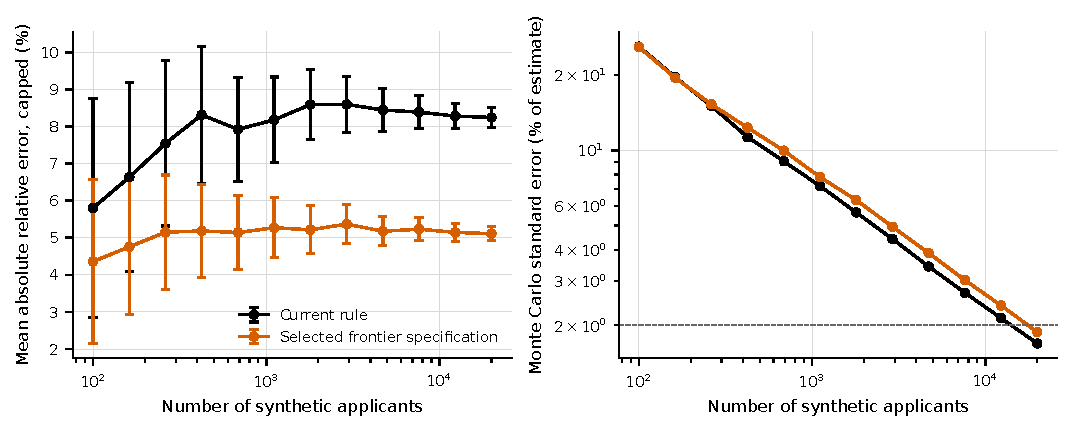
\includegraphics[width=\linewidth]{figures/si_convergence}
\caption{Synthetic data. (a) Running estimate of the accuracy loss with 95\% intervals and
(b) its Monte Carlo standard error relative to the estimate (dashed line at 2\%).}\label{fig:conv}
\end{figure}

\paragraph{Empirical validity.} Not established. No REAP application microdata under the
revised rule exist, and we found no openly downloadable dataset of metered pre- and
post-retrofit periods with known savings for comparable facilities; the Building Data
Genome Project 2 \cite{miller2020building} has no retrofit labels.

\section{Additional results}

{\scriptsize
\begin{longtable}{p{0.36\linewidth}llrrrrr}
\caption{Synthetic data: absolute relative error (\%) of the verified quantity by specification and condition (E2).}\label{tab:acc-full}\\
\hline
Specification & Condition & Type & 5th & Median & 95th & MARE & $>10\%$ \\
\hline
\endfirsthead
\hline
Specification & Condition & Type & 5th & Median & 95th & MARE & $>10\%$ \\
\hline
\endhead
Current rule: monthly quantities, annual claim & Clean & RES & 0.03 & 0.33 & 1.0 & 0.4 & 0.0 \\
Current rule: monthly quantities, annual claim & Clean & EEI & 2.04 & 22.85 & 100.1 & 31.2 & 74.9 \\
Current rule: monthly quantities, annual claim & Validated & RES & 0.03 & 0.35 & 1.2 & 1.0 & 2.6 \\
Current rule: monthly quantities, annual claim & Validated & EEI & 2.05 & 23.80 & 130.3 & 33.4 & 75.5 \\
Current rule: monthly quantities, annual claim & Unvalidated & RES & 0.04 & 0.40 & 69.4 & 8.3 & 13.7 \\
Current rule: monthly quantities, annual claim & Unvalidated & EEI & 2.15 & 25.53 & 228.4 & 36.5 & 76.6 \\
+ billing-period dates & Clean & RES & 0.03 & 0.33 & 1.0 & 0.4 & 0.0 \\
+ billing-period dates & Clean & EEI & 1.99 & 22.47 & 97.3 & 30.7 & 75.0 \\
+ billing-period dates & Validated & RES & 0.03 & 0.35 & 1.2 & 1.0 & 2.6 \\
+ billing-period dates & Validated & EEI & 2.05 & 23.48 & 130.3 & 33.1 & 75.7 \\
+ billing-period dates & Unvalidated & RES & 0.04 & 0.40 & 69.4 & 8.3 & 13.7 \\
+ billing-period dates & Unvalidated & EEI & 2.09 & 24.99 & 227.0 & 36.1 & 76.6 \\
+ dates and weather normalization & Clean & RES & 0.03 & 0.33 & 1.0 & 0.4 & 0.0 \\
+ dates and weather normalization & Clean & EEI & 1.15 & 15.25 & 76.8 & 23.1 & 63.9 \\
+ dates and weather normalization & Validated & RES & 0.03 & 0.35 & 1.2 & 1.0 & 2.6 \\
+ dates and weather normalization & Validated & EEI & 1.22 & 16.20 & 117.2 & 25.9 & 65.0 \\
+ dates and weather normalization & Unvalidated & RES & 0.04 & 0.40 & 69.4 & 8.3 & 13.7 \\
+ dates and weather normalization & Unvalidated & EEI & 1.29 & 17.23 & 245.6 & 29.5 & 66.7 \\
+ dates, normalization, read type & Clean & RES & 0.03 & 0.33 & 1.0 & 0.4 & 0.0 \\
+ dates, normalization, read type & Clean & EEI & 1.05 & 14.50 & 69.3 & 21.5 & 61.9 \\
+ dates, normalization, read type & Validated & RES & 0.03 & 0.35 & 1.2 & 1.0 & 2.6 \\
+ dates, normalization, read type & Validated & EEI & 1.11 & 15.23 & 102.0 & 24.3 & 63.1 \\
+ dates, normalization, read type & Unvalidated & RES & 0.04 & 0.40 & 69.4 & 8.3 & 13.7 \\
+ dates, normalization, read type & Unvalidated & EEI & 1.14 & 16.26 & 226.9 & 27.9 & 64.7 \\
+ monthly production-meter readings & Clean & RES & 0.03 & 0.33 & 1.0 & 0.4 & 0.0 \\
+ monthly production-meter readings & Clean & EEI & 2.04 & 22.85 & 100.1 & 31.2 & 74.9 \\
+ monthly production-meter readings & Validated & RES & 0.03 & 0.34 & 1.0 & 0.4 & 0.0 \\
+ monthly production-meter readings & Validated & EEI & 2.05 & 23.80 & 130.3 & 33.4 & 75.5 \\
+ monthly production-meter readings & Unvalidated & RES & 0.03 & 0.35 & 1.4 & 4.2 & 3.9 \\
+ monthly production-meter readings & Unvalidated & EEI & 2.15 & 25.53 & 228.4 & 36.5 & 76.6 \\
+ post-installation bills with export and netting basis & Clean & RES & 0.03 & 0.33 & 1.0 & 0.4 & 0.0 \\
+ post-installation bills with export and netting basis & Clean & EEI & 2.04 & 22.85 & 100.1 & 31.2 & 74.9 \\
+ post-installation bills with export and netting basis & Validated & RES & 0.03 & 0.35 & 1.2 & 1.0 & 2.5 \\
+ post-installation bills with export and netting basis & Validated & EEI & 2.05 & 23.80 & 130.3 & 33.4 & 75.5 \\
+ post-installation bills with export and netting basis & Unvalidated & RES & 0.04 & 0.40 & 69.4 & 8.3 & 13.7 \\
+ post-installation bills with export and netting basis & Unvalidated & EEI & 2.15 & 25.53 & 228.4 & 36.5 & 76.6 \\
Monthly data with metadata (dates, normalization, read type, & Clean & RES & 0.03 & 0.33 & 1.0 & 0.4 & 0.0 \\
Monthly data with metadata (dates, normalization, read type, & Clean & EEI & 1.05 & 14.50 & 69.3 & 21.5 & 61.9 \\
Monthly data with metadata (dates, normalization, read type, & Validated & RES & 0.03 & 0.34 & 1.0 & 0.4 & 0.0 \\
Monthly data with metadata (dates, normalization, read type, & Validated & EEI & 1.08 & 14.48 & 69.3 & 21.5 & 61.8 \\
Monthly data with metadata (dates, normalization, read type, & Unvalidated & RES & 0.03 & 0.35 & 1.4 & 4.2 & 3.9 \\
Monthly data with metadata (dates, normalization, read type, & Unvalidated & EEI & 1.14 & 16.26 & 226.9 & 27.9 & 64.7 \\
Interval data (utility and production) with normalization & Clean & RES & 0.03 & 0.33 & 1.0 & 0.4 & 0.0 \\
Interval data (utility and production) with normalization & Clean & EEI & 0.91 & 12.07 & 60.3 & 18.6 & 55.6 \\
Interval data (utility and production) with normalization & Validated & RES & 0.03 & 0.33 & 1.0 & 0.4 & 0.0 \\
Interval data (utility and production) with normalization & Validated & EEI & 0.91 & 12.07 & 60.3 & 18.6 & 55.6 \\
Interval data (utility and production) with normalization & Unvalidated & RES & 0.03 & 0.33 & 1.0 & 0.4 & 0.0 \\
Interval data (utility and production) with normalization & Unvalidated & EEI & 0.91 & 12.07 & 60.3 & 18.6 & 55.6 \\
\hline
\end{longtable}

}

\begin{table}[h]
\caption{Pre-specified paired Wilcoxon signed-rank tests on absolute relative error
(error-free synthetic evidence), with Holm correction.}\label{tab:tests}
\centering\footnotesize
\begin{tabular}{lp{0.5\linewidth}rrrr}
\hline
 & Comparison (a vs b) & $n$ & Median a (\%) & Median b (\%) & Holm $p$ \\
\hline
H1 & Dated monthly bills with normalization vs interval data (EEI absolute relative error) & 4457 & 15.2 & 12.1 & $<0.001$ \\
H2 & Normalized vs unnormalized dated monthly bills (EEI absolute relative error) & 4457 & 15.2 & 22.5 & $<0.001$ \\
H3 & Dated vs undated monthly bills (EEI absolute relative error) & 4457 & 22.5 & 22.8 & $<0.001$ \\
H4 & Dated vs undated pre-period consumption (absolute relative error) & 20000 & 0.3 & 0.4 & $<0.001$ \\
\hline
\end{tabular}

\end{table}

\begin{table}[h]
\caption{Synthetic data. Median absolute relative error (\%) of EEI savings estimators on
error-free evidence by true savings fraction ($n=\BandLowN$, \BandMidN, \BandHighN).}
\label{tab:bands}
\centering\footnotesize
\begin{tabular}{lrrr}
\hline
Estimator & below 10\% & 10-20\% & above 20\% \\
\hline
dated & 32 & 19 & 17 \\
interval & 15 & 9 & 13 \\
normalized guarded & 19 & 13 & 15 \\
normalized merged & 17 & 12 & 15 \\
normalized monthly & 19 & 13 & 15 \\
undated & 33 & 19 & 17 \\
\hline
\end{tabular}

\end{table}

{\footnotesize\setlength{\tabcolsep}{3.5pt}
\begin{longtable}{rrlrrrr}
\caption{Synthetic data: error with missing or estimated billing periods (E5).}\label{tab:e5}\\
\hline
Estimated reads (\%) & Missing months & Estimator & $n$ & Median ARE (\%) & 95th pct. (\%) & Date rules flag (\%) \\
\hline
\endfirsthead
\hline
Estimated reads (\%) & Missing months & Estimator & $n$ & Median ARE (\%) & 95th pct. (\%) & Date rules flag (\%) \\
\hline
\endhead
0 & 0 & s\_undated & 332 & 22.0 & 109 & 0 \\
0 & 0 & s\_dated & 332 & 22.2 & 100 & 0 \\
0 & 0 & s\_norm & 332 & 15.0 & 66 & 0 \\
0 & 0 & s\_norm\_merged & 332 & 15.0 & 66 & 0 \\
0 & 0 & cpre\_undated & 1500 & 0.4 & 2 & 0 \\
0 & 0 & cpre\_dated & 1500 & 0.2 & 2 & 0 \\
0 & 1 & s\_undated & 332 & 33.2 & 148 & 100 \\
0 & 1 & s\_dated & 332 & 34.2 & 160 & 100 \\
0 & 1 & s\_norm & 332 & 18.7 & 130 & 100 \\
0 & 1 & s\_norm\_merged & 332 & 18.7 & 130 & 100 \\
0 & 1 & cpre\_undated & 1500 & 7.8 & 19 & 100 \\
0 & 1 & cpre\_dated & 1500 & 1.7 & 12 & 100 \\
0 & 2 & s\_undated & 332 & 37.0 & 153 & 100 \\
0 & 2 & s\_dated & 332 & 40.2 & 181 & 100 \\
0 & 2 & s\_norm & 332 & 18.2 & 156 & 100 \\
0 & 2 & s\_norm\_merged & 332 & 18.2 & 156 & 100 \\
0 & 2 & cpre\_undated & 1500 & 16.3 & 30 & 100 \\
0 & 2 & cpre\_dated & 1500 & 2.3 & 19 & 100 \\
0 & 3 & s\_undated & 332 & 36.8 & 171 & 100 \\
0 & 3 & s\_dated & 332 & 41.5 & 226 & 100 \\
0 & 3 & s\_norm & 332 & 22.2 & 251 & 100 \\
0 & 3 & s\_norm\_merged & 332 & 22.2 & 251 & 100 \\
0 & 3 & cpre\_undated & 1500 & 24.8 & 41 & 100 \\
0 & 3 & cpre\_dated & 1500 & 2.7 & 26 & 100 \\
10 & 0 & s\_undated & 332 & 23.1 & 108 & 0 \\
10 & 0 & s\_dated & 332 & 22.5 & 105 & 0 \\
10 & 0 & s\_norm & 332 & 19.0 & 88 & 0 \\
10 & 0 & s\_norm\_merged & 332 & 16.2 & 74 & 0 \\
10 & 0 & cpre\_undated & 1500 & 0.5 & 3 & 0 \\
10 & 0 & cpre\_dated & 1500 & 0.3 & 3 & 0 \\
30 & 0 & s\_undated & 332 & 24.8 & 118 & 0 \\
30 & 0 & s\_dated & 332 & 24.6 & 108 & 0 \\
30 & 0 & s\_norm & 332 & 24.4 & 175 & 0 \\
30 & 0 & s\_norm\_merged & 332 & 21.0 & 102 & 0 \\
30 & 0 & cpre\_undated & 1500 & 0.6 & 4 & 0 \\
30 & 0 & cpre\_dated & 1500 & 0.4 & 4 & 0 \\
50 & 0 & s\_undated & 332 & 26.5 & 123 & 0 \\
50 & 0 & s\_dated & 332 & 26.5 & 116 & 0 \\
50 & 0 & s\_norm & 332 & 30.1 & 225 & 0 \\
50 & 0 & s\_norm\_merged & 332 & 22.0 & 112 & 0 \\
50 & 0 & cpre\_undated & 1500 & 0.7 & 5 & 0 \\
50 & 0 & cpre\_dated & 1500 & 0.6 & 5 & 0 \\
\hline
\end{longtable}

}

\begin{figure}[h]
\centering
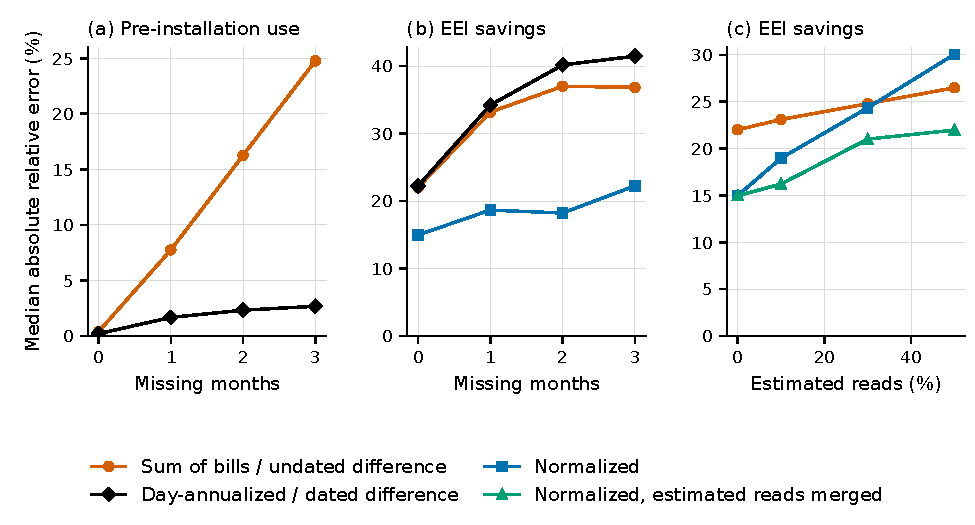
\includegraphics[width=\linewidth]{figures/si_incomplete}
\caption{Synthetic data ($n=\EFiveN$ applicants per condition). Median error (a, b) with
missing months per period and (c) with estimated reads.}\label{fig:e5}
\end{figure}

\begin{table}[h]
\caption{Synthetic data, hypothetical element times. Respondent time and losses by
collection mode when the mode is available to all respondents.}\label{tab:modes}
\centering\footnotesize\setlength{\tabcolsep}{4pt}
\begin{tabular}{llrrrr}
\hline
Specification & Collection mode & Minutes & 90\% interval & MARE (\%) & Selection change (\%) \\
\hline
current & Manual transcription & 166 & 164--170 & 8.2 & 9.2 \\
current & Utility file upload & 103 & 82--132 & 8.2 & 9.2 \\
current & Green Button download & 103 & 82--132 & 8.2 & 9.2 \\
current & Automated utility data access & 82 & 64--104 & 8.2 & 9.2 \\
recommended & Manual transcription & 230 & 211--255 & 5.1 & 4.7 \\
recommended & Utility file upload & 133 & 107--171 & 5.1 & 4.7 \\
recommended & Green Button download & 133 & 107--171 & 5.1 & 4.7 \\
recommended & Automated utility data access & 112 & 89--143 & 5.1 & 4.7 \\
recommended interval & Manual transcription & 256 & 228--340 & 4.5 & 4.0 \\
recommended interval & Utility file upload & 192 & 156--291 & 4.5 & 4.0 \\
recommended interval & Green Button download & 129 & 104--166 & 4.5 & 4.0 \\
recommended interval & Automated utility data access & 108 & 85--138 & 4.5 & 4.0 \\
metadata & Manual transcription & 278 & 251--319 & 5.1 & 4.7 \\
metadata & Utility file upload & 146 & 120--191 & 5.1 & 4.7 \\
metadata & Green Button download & 146 & 120--192 & 5.1 & 4.7 \\
metadata & Automated utility data access & 125 & 102--163 & 5.1 & 4.7 \\
interval & Manual transcription & 262 & 234--351 & 4.5 & 4.1 \\
interval & Utility file upload & 199 & 163--300 & 4.5 & 4.1 \\
interval & Green Button download & 136 & 110--180 & 4.5 & 4.1 \\
interval & Automated utility data access & 115 & 91--150 & 4.5 & 4.1 \\
\hline
\end{tabular}

\end{table}

\begin{figure}[h]
\centering
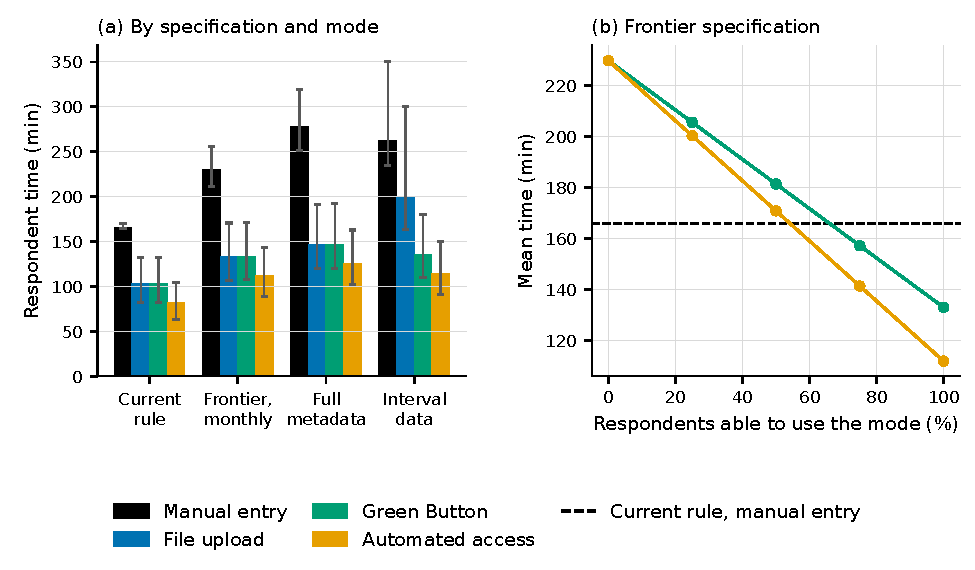
\includegraphics[width=\linewidth]{figures/si_modes}
\caption{Hypothetical element times. (a) Respondent time by collection mode, with 90\%
Monte Carlo intervals, and (b) mean time for the monthly-data frontier specification as a
function of the share of respondents able to use a mode.}\label{fig:modes}
\end{figure}

\begin{table}[h]
\caption{Synthetic data ($n=\SizeSensN$ applicants per scenario). Sensitivity to assumed
load noise (multipliers \NoiseLowDailySd/\NoiseCentralDailySd/\NoiseHighDailySd\% daily s.d.)
and probability of a non-routine change: median absolute relative error (\%) of EEI
savings estimators against normal-year savings, share above \ErrorShareThreshold\% for
the undated difference, and share of awards changed with error-free evidence under the
current elements. By origin of the load shape, the undated median error is
\BasisComstockUndatedMedian\% (ComStock types, $n=\BasisComstockN$) and
\BasisHypotheticalUndatedMedian\% (hypothetical agricultural types,
$n=\BasisHypotheticalN$); interval data give \BasisComstockIntervalMedian\% and
\BasisHypotheticalIntervalMedian\%.}\label{tab:noise}
\centering\footnotesize\setlength{\tabcolsep}{2.5pt}
\begin{tabular}{lrrrrrrr}
\hline
Scenario & Daily noise s.d. & Non-routine change & Undated & Dated, adjusted & Interval & Undated $>10\%$ & Awards changed \\
\hline
central & 6 & 15 & 21 & 15 & 11 & 74 & 6.3 \\
low & 3 & 0 & 21 & 11 & 9 & 72 & 5.6 \\
high & 12 & 30 & 25 & 20 & 16 & 78 & 6.2 \\
\hline
\end{tabular}

\end{table}

\begin{table}[h]
\caption{Sobol indices (Saltelli sampling, $N=\SobolN$ base samples, bootstrap
confidence half-widths) of the difference in respondent time between the monthly-data
frontier specification and the current specification (mean \SobolOutputMean{} min, s.d.\
\SobolOutputSd{} min over the time distributions).}\label{tab:sobol}
\centering\footnotesize
\begin{tabular}{lrrrr}
\hline
Time parameter & $S_1$ & $\pm$ & $S_T$ & $\pm$ \\
\hline
required.locate\_bills & 0.282 & 0.024 & 0.297 & 0.016 \\
optional.inverter\_monthly.fixed & 0.258 & 0.021 & 0.263 & 0.015 \\
required.energy\_price & 0.128 & 0.016 & 0.139 & 0.008 \\
optional.billing\_dates.per\_bill & 0.105 & 0.014 & 0.107 & 0.006 \\
required.bill\_energy\_per\_bill & 0.068 & 0.012 & 0.076 & 0.005 \\
optional.meter\_ids.fixed & 0.054 & 0.010 & 0.056 & 0.003 \\
required.annual\_claim & 0.033 & 0.009 & 0.036 & 0.002 \\
optional.read\_type.per\_bill & 0.029 & 0.007 & 0.030 & 0.002 \\
rework & 0.018 & 0.006 & 0.018 & 0.001 \\
required.rated\_capacity & 0.002 & 0.002 & 0.002 & 0.000 \\
\hline
\end{tabular}

\end{table}

\bibliographystyle{unsrturl}
\bibliography{references}
\end{document}
